\documentclass[12pt,a4paper,twoside]{book}
\usepackage{graphicx}
\usepackage{setspace}	%double spacing for text, single for captions, footnotes, etc.
%\usepackage{hypernat} 	%substitut de cite que permet fer hyperlinks
\usepackage{natbib}		% substituye a 'hypernat' que funciona en Windows.
\usepackage[english]{babel}
\usepackage[utf8]{inputenc}
\usepackage{color}
\usepackage[dvipsnames, table]{xcolor}
\usepackage{hhline} 		% extended styles for tables
\usepackage{multirow}
\usepackage{subfigure}
\usepackage{acronym}
\usepackage{hyperref}
\usepackage{amsmath,amsmath,amssymb} 
\usepackage{fancyhdr}
\usepackage{epsfig, amsmath}
\usepackage{algorithm}
\usepackage{algorithmic}
\usepackage{pgfgantt}
\usepackage{placeins}

\usepackage{tcolorbox}
\usepackage{tabularx}


\RequirePackage{booktabs}

% general settings
\hypersetup{
	linktocpage=true,
	colorlinks=true,
	linkcolor=blue,
	citecolor=blue,
}
\definecolor{Hgray}{gray}{0.6}

\newenvironment{definition}[1][Definition]{\begin{trivlist}
\item[\hskip \labelsep {\bfseries #1}]}{\end{trivlist}}


%
% Nuevo comando para resaltar nombres de archivo.
\newcommand{\filename}[1]{\texttt{#1}}

%
% Nuevo comando para URLs.
\newcommand{\myurl}[2]{\href{#1}{#2}\footnote{\url{#1}}}

%
% Imagenes
\newcommand{\imagen}[3][0.8]{
	\begin{figure}[!ht]
		\centering
		\includegraphics[width=#1\textwidth]{#2}
		\caption{#3}\label{fig:#2}
	\end{figure}
	%\FloatBarrier
}

%
% Tabla
\newcolumntype{C}{>{\arraybackslash}X} % centered "X" column

%
% Red color for to be done or to be replaced things in document
\newcommand{\TBD}[1]{\textcolor{BrickRed}{#1}}

%
%Paragraph formatting
\setlength{\topmargin}{0cm}
\setlength{\textheight}{23cm}
\setlength{\textwidth}{17cm}
\setlength{\oddsidemargin}{0cm}
\setlength{\evensidemargin}{0cm}
\setlength{\headheight}{1cm}

% indica que las 'sub-sub-sections' sean numeradas y aparezcan en el indice
\setcounter{secnumdepth}{3}
\setcounter{tocdepth}{3}

% settings for code
\renewcommand{\algorithmicrequire}{\textbf{Entrada: }}
\renewcommand{\algorithmicensure}{\textbf{Salida: }}

%%%%%%%%%%%%
% DOCUMENT %
%%%%%%%%%%%%
\begin{document}

% portada
\newpage
\thispagestyle{empty}

\baselineskip 2em

%\vspace*{1cm}

\centerline{
\includegraphics[width=0.6\textwidth]{images/UOC-logo}}
\begin{center}
\textsc{Universitat Oberta de Catalunya (UOC) \\
 Masters in Data Science\\}

%\centerline {\pic{UOC}{4cm}}

\vspace*{1.5cm}

\textsc{\Large MASTER'S THESIS}

\vspace*{0.5cm}

\textsc{\large Area: Medicine Area (TFM-Med)}


%\textbf{\Huge VirtualTechLab Model: }

\vspace*{2.0cm}

\textbf{\Large Deep Convolutional Autoencoder for control brain MRI}

\textbf{\large Development and Applications}

\vspace{2.5cm}
\baselineskip 1em

\baselineskip 2em
-----------------------------------------------------------------------------\\
Author:     Adrián Arnaiz Rodríguez\\
Tutor:      Baris Kanber\\
TFM Professor: Ferran Prados Carrasco\\
-----------------------------------------------------------------------------\\
\vspace*{1.5cm}
Barcelona, \today

\end{center}

\newpage
\pagestyle{empty}
\hfill

\newpage
% abstract
\pagenumbering{roman} 
\setcounter{page}{1} 
\pagestyle{plain}

%%%%%%%%%%%%%%%%
%%% CREDITOS %%%
%%%%%%%%%%%%%%%%
\chapter*{Créditos/Copyright}

\vspace{1cm}

\begin{figure}[ht]
    \centering
	
\includegraphics[scale=1]{images/license.png}
\end{figure}

Este obra está bajo una \href{http://creativecommons.org/licenses/by-nc-sa/3.0/es/}{licencia de Creative Commons \textit{Reconocimiento, NoComercial, CompartirIgual} 3.0 España}.

\begin{figure}[ht]
    \centering
	
\includegraphics[scale=1]{images/license.png}
\end{figure}

This work is licensed under a \href{http://creativecommons.org/licenses/by-nc-sa/3.0/es/deed.en}{Creative Commons Attribution-NonCommercial-ShareAlike 3.0 Spain License}.

The \myurl{https://github.com/AdrianArnaiz/Brain-MRI-Autoencoder}{official code repository of this Master's Thesis} is licensed under MIT license.

%%%%%%%%%%%%%
%%% FICHA %%%
%%%%%%%%%%%%%
\chapter*{FICHA DEL TRABAJO FINAL}

\begin{table}[ht]
	\centering{}
	\renewcommand{\arraystretch}{2}
	\begin{tabular}{r | l}
		\hline
		Título del trabajo: & \vtop{\hbox{\strut Deep Convolutional Autoencoders  } \hbox{\strut for reconstructing magnetic }\hbox{\strut resonance images of the healthy brain}}\\
		\hline
        Nombre del autor: & Adrián Arnaiz Rodríguez\\
		\hline
        Nombre del colaborador/a docente: & Baris Kanber\\
		\hline
        Nombre del PRA: & Ferrán Prados Carrasco\\
		\hline
        Fecha de entrega (mm/aaaa): & 01/2021\\
		\hline
        Titulación o programa: & Máster en Ciencia de Datos\\
		\hline
        Área del Trabajo Final: & Area Medicina (TFM-Med)\\
		\hline
        Language: & English\\
		\hline
        Keywords & Deep Learning, Brain MRI, Autoencoder\\
		\hline
	\end{tabular}
\end{table}

%%%%%%%%%%%%%%%%%%%
%%% DEDICATORIA %%%
%%%%%%%%%%%%%%%%%%%
\chapter*{}

\epigraph{{\Large Nobody ever figures out what life is all about, and it doesn't matter. Explore the world. Nearly everything is really interesting if you go into it deeply enough}}{{\large Richard P. Feynman}}

%%%%%%%%%%%%%%%%%%%
%%% Agradecimientos %%%
%%%%%%%%%%%%%%%%%%%
\chapter*{Acknowledgment}

I would like to express my special thanks and gratitude to my Master's Thesis Director, Baris Kanber, who has been widely open to solve all my doubts and also discussing the proposed approaches of the project. He also has encouraged me to do my best and provide me the opportunity to prepare the project.

I would also like to extend my gratitude to all the professors that I have had in this Master's, which despite being online, they have been very close to us for everything we need.

I also pay my deep sense of gratitude to the professors of ADMIRABLE research group of the University of Burgos. They let me focus on the Master's Degree to finish it as soon as possible, sometimes even allowing me to set aside some group research assignments.

Last, but not least, my family is also an inspiration and a big support for me.


%%%%%%%%%%%%%%%%
%%% RESUMEN  %%%
%%%%%%%%%%%%%%%%
\chapter*{\centering Abstract}
\addcontentsline{toc}{chapter}{Abstract}

\onehalfspacing

\begin{quote}
{The analysis of brain MRI is critical for a proper diagnosis and treatment of neurological diseases. Improvements in this field lead to better health quality. Numerous branches can be still enhanced due to the nature of MRI recompilation: disease detection and segmentation, data augmentation, improvement in data collection, or image enhancement are some of them.

For several years, many approaches have been taken to address this. Machine Learning and Deep Learning emerge as very popular approaches to solve problems. Several kinds of data mining problems (supervised, unsupervised, dimension reduction, generative models, etc) and algorithms can be applied to the problem-solving of MRI. Besides, new emerging deep learning architectures for another kind of image task can be helpful. New types of convolution, autoencoders or generative adversarial networks are some of them.

Therefore, the purpose of this work is to apply one of these new techniques to T1 weighted brain MRI. We will develop a Deep Convolutional Autoencoder, which can be used to help some problems with neuroimaging. The input of the Autoencoder will be control T1WMRI and aims to return the same image, with the problematic that, inside its architecture, the image travels through a lower-dimensional space, so the reconstruction of the original image becomes more difficult. Thus, the Autoencoder represents a normative model.

This normative model will define a distribution (or normal range) for the neuroanatomical variability for the illness absence. Once trained with these control images, we will discuss the potential application of the autoencoder like noise reducer or disease detector.}
\end{quote}

%{http://www.ece.cmu.edu/~koopman/essays/abstract.html}
%{http://www.ece.cmu.edu/~koopman/essays/abstract.html}

\textbf{Keywords}: Deep Learning, Brain MRI, Deep Convolutional Autoencoder, Image denoising.

\clearpage

\chapter*{\centering Resumen}

\addcontentsline{toc}{chapter}{Resumen}

\begin{quote}
{El análisis de las resonancias magnéticas cerebrales es fundamental para un diagnóstico y tratamiento adecuados de las enfermedades neurológicas. Se pueden mejorar ámbitos del análisis debido a la naturaleza de la recopilación de resonancias: detección y segmentación de enfermedades, aumento de datos, mejora en la extracción o mejora de imágenes.

El aprendizaje automático y el aprendizaje profundo surgen como nuevas alternativas populares para resolver estos problemas. Se pueden aplicar varios enfoques de minería de datos y algoritmos para la resolución de problemas relacionados con la neuroimagen (supervisados, no supervisados, reducción de dimensionalidad, modelos generativos, etc.). Además, las nuevas arquitecturas emergentes de aprendizaje profundo, desarrolados para otro tipo de tareas de imagen, pueden ser útiles. Algunas de ellas son nuevos tipos de convolución, autoencoders o GAN.

Por lo tanto, el propósito de este trabajo es aplicar una de estas nuevas técnicas a resonancias cerebrales tipo T1. Desarrollaremos un Autoencoder convolucional profundo, que puede usarse para ayudar con algunos problemas de neuroimagen. La entrada del Autoencoder será el imágenes de control T1WMRI y tendrá como objetivo devolver la misma imagen, con la problemática de que, dentro de su arquitectura, la imagen viaja por un espacio de menor dimensión, por lo que la reconstrucción de la imagen original se vuelve más difícil. El autoencoder representa un modelo normativo.

Este modelo normativo definirá una distribución (o rango normal) para la variabilidad neuroanatómica para la ausencia de enfermedad. Una vez entrenado con imágenes de control, discutiremos la aplicación potencial del Autoencoder como reductor de ruido o detector de enfermedades.

}
\end{quote}
\textbf{Keywords}: Aprendizaje profundo, Imágenes cerebrales de resonancias magnéticas, Autoencoder convolucional profundo, eliminación de ruido de imágenes.



\clearpage
\newpage

\pagestyle{fancy}
\renewcommand{\chaptermark}[1]{ \markboth{#1}{}}
\renewcommand{\sectionmark}[1]{\markright{ \thesection.\ #1}}
\lhead[\fancyplain{}{\bfseries\thepage}]{\fancyplain{}{\bfseries\rightmark}}
\rhead[\fancyplain{}{\bfseries\leftmark}]{\fancyplain{}{\bfseries\thepage}}
\cfoot{}

% indice
\cleardoublepage
\phantomsection
\addcontentsline{toc}{chapter}{Content}
\tableofcontents
% listado de figuras
\cleardoublepage
\phantomsection
\addcontentsline{toc}{chapter}{List of Figures}
\listoffigures
% listado de tablas
\cleardoublepage
\phantomsection
\addcontentsline{toc}{chapter}{List of Tables}
\listoftables

\thispagestyle{empty}

\pagenumbering{arabic}

\pagestyle{fancy}
\renewcommand{\chaptermark}[1]{ \markboth{#1}{}}
\renewcommand{\sectionmark}[1]{\markright{ \thesection.\ #1}}
\lhead[\fancyplain{}{\bfseries\thepage}]{\fancyplain{}{\bfseries\rightmark}}
\rhead[\fancyplain{}{\bfseries\leftmark}]{\fancyplain{}{\bfseries\thepage}}
\cfoot{}

%http://kb.mit.edu/confluence/pages/viewpage.action?pageId=3907092
\onehalfspacing
\setlength{\parskip}{1em}
\rmfamily

% capitulos del documento
\chapter{Introduction}
\label{chapter:introduccion}

\textit{Not Final Note: \TBD{This color ('TBD' tag in latex) are going to be used in non-final versions of the memory to highlight the non-final sentences or things to be changed in the final version}}.

In this chapter we will introduce the main background, and aims of the project, basing it on its non-solved tasks and relevance.

%%% SECTION
\section{Problem overview and relevance}

\subsection{MRI general problems}

Neuroimaging in medicine allows studying the morphological features of the human brain. With the objective of improving the detection systems, diagnostic and treatment, correlations between the morphological features and the neurological disorders can be addressed in order to achieve that \cite{abou2006neuroimaging}. If we improve brain magnetic resonance image analysis \ref{fig:figs/MRI_image.jpg}, we will improve the detection systems and treatments for neurological diseases, so the social relevance of the field is very important.

\imagen{figs/MRI_image.jpg}{Brain MRI examples \cite{fotomri}}

The relevance of the project is also shown that there are a lot of branches in which neuroimaging analysis can improve. Machine learning, and more recently Deep Learning and Computer Vision, has irrupted in this field for helping in some tasks: 

\begin{itemize}
    \item \textbf{Disease detection: segmentation and classification}. There are still several problems to solve in classification and segmentation problems. Brain MRIs are high dimensional, so we have to recruit big amount of images to properly develop a Machine Learning model that be able to achieve high accuracy. It is very difficult to recruit a large number of images, especially disease images. Even if it performs well, machine learning algorithms have been criticized due to the difficult of extract a clear knowledge of them (black-boxes).  \cite{myronenko20183d}. So a experimental approach is disease detection based on outliers from a normative model Patients with pathologies will be outliers in the distribution build by the normative model (they will be out of normal range defined by the normative model) \cite{marquand2016normative} \cite{mourao2011outlier}.
    \item \textbf{Data Augmentation}. Lack of data problem can be addressed by Data Augmentation techniques, which look for improve our Machine Learning models \cite{GanDataAugment2018}.
    \item \textbf{Improvement of data collection}. Recently high-impact \myurl{https://fastmri.org/}{FastMRI} release from Facebook for improving the speed in MRI scans \cite{fastmri}.
    \item \underline{\textbf{Image enhancement}}. Clinical evaluation is critical for good disease treatment. Experts and algorithms need good quality images to carry out their tasks. This is a problem we want to address, so we will explain it deeper in the document \cite{tamada2020review} \cite{myronenko20183d}. 
\end{itemize}

\subsection{MRI Image enhancement}

\textbf{We are going to focus on the problem of image enhancement, specifically the problem of noise removal}, see \ref{fig:figs/Denoised_MRI.jpeg}. If we achieved good performance in this task, we would research about how to apply this solution to disease detection or data augmentation.

\imagen{figs/Denoised_MRI.jpeg}{Noised and Denoised MRI \cite{fotoDenoisedMri}}

Magnetic resonance images are collected with MR scans and the scan process, even though it is improved continually, adds some failures to the MR image. MR images have some random \textbf{noise} and \textbf{artifacts} due to this fact \cite{artifacts86}. This noise and artifacts are present in the image due to different reasons: hardware-reasons (magnetic fields, etc.), body motion during scanning, thermal noise, weak signal intensity (which causes low signal-to-noise ratio), etc. The difference between noise and artifact is that noise can hide the characteristics of an image, whereas artifacts appear to be characteristic but are not. If the 'problem' is structured, it is probably an artifact, while if it is random, it is probably noise.

\subsection{Noise and artifact reduction with Deep Learning}

To address this problem many approaches have been done, all of them with some disadvantages. Advanced filtering methods \cite{filtermeth12} or retrospective correction approaches have been proposed, but, with the rise of \textbf{Deep Learning}, other methods have been proposed that take advantage of this approach. Deep Learning is very powerful in high-dimensional spaces and non-linear problems, so it can make a better job in feature extraction or information compression. Therefore, it will have good performance with images, where the \textbf{underlying structure of the images will be captured and foreign elements such as noise or artifacts can be eliminated}. 

There are some approaches to reduce the noise and artifacts in MRI images. An recent and outstanding review is made by D.Tamada \cite{tamada2020review}. In this paper D.Tamada summarize Deep Learning Architectures and applications to MRI. We notice the big relevance of denoiser MRI Deep Learning methods in this review. Although there are many methods, we will focus in brain MRI denoisers. 

There are some Deep Learning Architectures to address in the problem of denoise an brain MRI: Single-scale CNN, Denoising CNN, Autoencoders, and GAN-based architectures. \textbf{We will choose the Autoencoder Architecture for this project}.

\textbf{Autoencoders} \cite{autoencoder} encode the input into a lower-dimensional space. It extracts important information from the higher-dimensional space, encodes it, and then decodes it to reconstruct the higher-dimensional spacer from the lower one. \TBD{This architecture will be deeply explained in \ref{chapter:theory} in further stages of the project.}



\subsection{Our approach}

\begin{tcolorbox}
In this project, we will design a \textbf{Deep Learning autoencoder for reconstructing brain magnetic resonance images removing noise. In other words, we will train a autoencoder with disease-free neuroimaging data and, with this trained autoencoder, we could define a distribution (or normal range) for the neuroanatomical variability for the illness absence with the main purpose of removing noise. Once trained, the autoencoder should be able to encode a input image and decode it removing noise.}
\end{tcolorbox}

\textbf{If the main objective of the project is completed, we could research the application of this model in data augmentation and disease detection fields}. In the case of \textbf{data augmentation}, we will then attempt to reconstruct magnetic resonance images from patients with brain pathologies, with a further view to using the autoencoder to generate 'pathology-free' versions of the said images. In the case of \textbf{disease detection}, we could take an approach like the one in \cite{pinaya2019} (creating a measure for the difference between input and output image and classify it as healthy or control based on this measure). Patients with pathologies will be outliers in the distribution build by the autoencoder (they will be out of normal range defined by the autoencoder) \cite{marquand2016normative} \cite{mourao2011outlier}. This assumption of patients as outliers (based in \cite{mourao2011outlier}) is used in \cite{pinaya2019} for abnormal brain structure detection.

Of course, we will need \textbf{data}. For this project, we will use \textbf{T1-weighted MRI images of control subjects} (no disease). As the project is of fairly limited length, we won't need to detect disease as a principal objective, but only learn to reconstruct normal MRI images, so we won't need pathology images for this project. In addition, we will investigate whether our method of reconstruction can filter out noise and/or artefacts. So, in essence, we will have $n$ 3D MRI volumes ($n$ can be any number greater than 100) from healthy subjects, we will preprocess it (data augmentation based on adding noise, remove parts...), and train our model to reconstruct the source MRI volumes. We will have access magnetic brain resonance images from control subjects for training the autoencoder. This data is arranged from different sources. \TBD{Concrete sources of data images used in the project will be discussed in further stages but we have some clear options in this moment}:

\begin{itemize}
    \item The \myurl{https://brain-development.org/ixi-dataset/}{IXI dataset} (\TBD{Most likely to be chosen}).
    \item Other data sources such as \myurl{https://openneuro.org}{Open Neuro}.
\end{itemize}



\section{Personal motivation}

My personal motivation to carry out the project arises from several factors. My first steps in the world of Machine Learning were in the last year of my career at the University of Burgos. I was lucky enough to collaborate last year with the \myurl{http://admirable-ubu.es/}{ADMIRABLE} research department. The project that I did (in which we continue working) was on the \myurl{https://adrianarnaiz.github.io/TFG-Neurodegenerative-Disease-Detection/}{use of biomarkers extracted from the voice for the construction of classifiers that detect Parkinson's disease}. The project include topics like \textbf{signal processing}, \textbf{supervised learning}, \textbf{unsupervised learning} and \textbf{transfer learning}. The project was very successful and we had a lot of impact at that time. We are currently in the process of meeting with the Burgos hospital to continue developing the model and the application (project and impact recompilation in \myurl{https://github.com/AdrianArnaiz/TFG-Neurodegenerative-Disease-Detection}{Github}).

This project has fully opened me the doors the world of artificial intelligence and machine learning, which is a field of knowledge that I love. I have always liked math, problem-solving and since I started my career I love programming. Therefore, I find this field the ideal that aligns with my tastes and interests. As I said before, I have done lot of jobs with supervised learning or data analysis, but only with tabular data sets or text-datasets, so I wanted to break in the world of image processing and Deep Learning.

Then I worked half year in Ernst and Young, developing Machine Learning systems for RPA tasks (classify emails at Telefónica, Chatbot for Maxium or Fuzzy Name Matching for Xunta de Galicia).

In addition, I believe that the application of AI to medicine is one of the fields that may be of greater general interest to society. By advancing in the speed and quality of medical diagnoses and treatments, it will be possible to achieve health of higher quality, speed and accessibility for all. Also, computer vision and deep learning have helped to achieve big advances in this field nowadays. 


\section{State of art: related works}
\textit{\TBD{In later stages of the project, the resume of related works and state of art will be replaced in other place of the document.}}

The world relevance and impact of this problem is also shown in the related articles of this subject. The state of art of Deep Learning Autoencoders applied to brain MRI shows the relevance of this field. \TBD{In this stage of the project (\today), we have deeply read 3 papers for building the first bricks and identify the goals and methodology of the project}.

\begin{itemize}
    \item Walter Pinaya, 2018 \cite{pinaya2019}:
    
    Classic methods and approaches based on sMRI (structural magnetic resonance imaging) can't get a good performance in abnormal brain structural detection because neuroanatomical alterations in neurological disorders can be subtle and spatially distributed. Another approach based on Machine Learning methods could improve performance. ML algorithms are sensitive to these subtle characteristics. The downside of this road is the need for a large amount of image data (control and disease) and that the models are black-boxes with no information on the critical characteristics used for the decision. With this Deep Autoencoder, they put this matter up for discussion.
    
    In this project, they address the problem of creating a normative model using a deep autoencoder trained with control subjects. With this autoencoder defining a distribution for control patients, they define a deviation metric to measure the neuroanatomical deviation in patients. Patients with some disorder should be outliers in this distribution.
    
    Architecture and technique used in the experiment:
    \begin{itemize}
        \item Semi-supervised autoencoder: reconstruction of the image and prediction of age and sex.
        \item 3 hidden layers with SELUs activation function.
        \item Output layer with Linear activation function.
        \item Loss function: MSE from reconstructed and original image + cross-entropy for age + cross-entropy for years + Unsupervised cross-covariance.
        \item 2000 epochs.
        \item ADAM optimizer (adaptive moment estimation) with adaptative learning rate.
        \item 64 samples mini-batches.
        \item Transformation of input image:
        \begin{itemize}
            \item Add Gaussian noise (0, 0.1).
            \item Feature scaling (normalization).
        \end{itemize}
        \item One-hot encoding for \texttt{sex} and \texttt{age} labels.
    \end{itemize}
    
    \item \TBD{We made a recompilation of papers reviewed in Table 1 of D. Tamada, 2020 \cite{tamada2020review} and by our own, with some removals and additions based in our goal of the project (see \ref{table:paper_overview}). In further stages we will explain deeply some papers from the table \ref{table:paper_overview}}. From the table of D. Tamada we only obtain 1 autoencoder study \cite{bermudez2018t1autoencoder}, 3 sCNN and DnCNN approaches \cite{kidoh2019scnnt1} \cite{ganHR3d} \cite{dncnnnoise2noise} and 1 GAN study. The other 5 papers have been compiled by our own (Autoencoder based: \cite{pinaya2019} \cite{gondara2016medicalautoencoder} \cite{superresolution} \cite{fuzzyautoencoder}, GAN-Autoencoder-based: \cite{wganautoencoder}).
    \item \TBD{In next stage (state of art research), we will research the state of art with new techniques and frameworks. \myurl{https://www.connectedpapers.com/}{Connected Papers} is a network science framework to improve the search of papers. There are also other platforms like \myurl{https://paperswithcode.com/}{Papers With Code} and \myurl{https://distill.pub/}{Distill} that improve the experience of article discovering and article visualization-interaction.}
\end{itemize}    

\begin{table}[!ht]
    \setlength\extrarowheight{2pt} % for a bit of visual "breathing space"
    \rowcolors {2}{gray!15}{}
    \begin{tabularx}{\textwidth}{C C C}
    \hline
        \textbf{Purpose} & \textbf{Year, Authors} & \textbf{Network} \\
        \hline
        
        \rowcolor{orange!10}
        \multicolumn{3}{c}{\textbf{Autoencoders}}\\
        
        \hline
        
        Identify brain abnormal structural patterns & 2018, W. Pinaya, et al \cite{pinaya2019} & \textbf{Semi-supervised autoencoder for HCP Dataset} \\
        
        Denoising for T1 weighted brain MRI & 2018, C. Bermudez, et al \cite{bermudez2018t1autoencoder} & \textbf{Autoencoder with skip connections} \\
        
        Medical image denoise & 2016, L. Gondara, et al \cite{gondara2016medicalautoencoder} &\textbf{Convolutional denoising autoencoder} \\
        
        General image denoising and super resolution & 2016, XJ. Mao et all \cite{superresolution} [Code available] & \textbf{Convolutional auto-encoders with symmetric skip connections} \\
        
        Brain MRI denoise & 2019, N. Chauhan et al \cite{fuzzyautoencoder} & \textbf{Convolutional denoising autoencoder with Fuzzy Logic filters} \\

        \hline
        \rowcolor{orange!10}
        \multicolumn{3}{c}{\textbf{sCNN and DnCNN}}\\
        \hline

        Denoising for T1, T2 and FLAIR brain images & 2018, M. Kidoh, et al \cite{kidoh2019scnnt1} & Single-scale CNN with DCT \\
        
        Motion artifact reduction for brain MRI & 2018, P. Johnson, et al \cite{scnnmotion} & Single-scale CNN\\
        
        Denoising for multishot DWI & 2020, M Kawamura et al \cite{dncnnnoise2noise} & DnCNN with Noise2Noise \\
        
        \hline
        \rowcolor{orange!10}
        \multicolumn{3}{c}{\textbf{GAN}}\\
        \hline
        
        Motion artifact reduction for brain MRI & 2018 BA. Duffy, et al \cite{ganHR3d} & GAN with HighRes3dnet as generator \\
        
        Denoise 3D MRI & 2019, M. Ran et al \cite{wganautoencoder} & \textbf{Wasserstein GAN with Convolutional Autoencoder generator} \\
 
    \hline
    \end{tabularx}
    \caption{Overview of studies for noise reduction based in Table 1 from D. Tamada \cite{tamada2020review} (In bold the autoencoder related architecture)}
    \label{table:paper_overview}
\end{table}

    


%%% SECTION NOT SHOWN, examples from tables and algorithms

\iffalse
\section{Latex Examples}

\begin{figure}
	\centering
	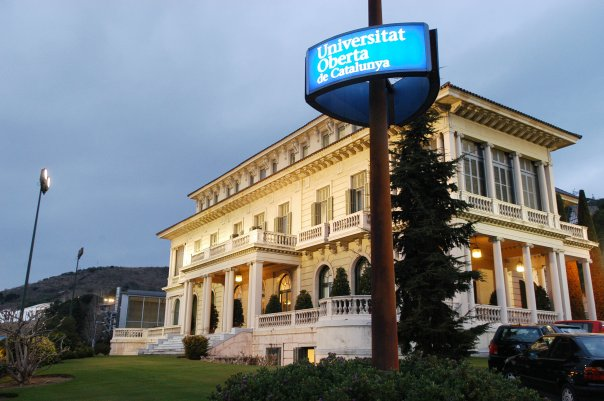
\includegraphics[width=0.6\textwidth]{figs/image1.png}
	\caption{Pie de la imagen.}
	\label{fig:context-anoni1}
\end{figure}


\imagen{figs/image1.png}{asdasd}

Un ejemplo de pseudo-código se puede encontrar en el Código \ref{code:RandomSwitch-1}

\begin{algorithm}
	\caption{Pseudocódigo del algoritmo \textit{Random Switch}}
	\label{code:RandomSwitch-1}
	\begin{algorithmic}
		\REQUIRE{El grafo original $G$ y el porcentaje de anonimización $p$ que se desea aplicar.}
		\ENSURE{El grafo $G$ anonimizado.}
		\STATE $num = round(G.num\_edges() * p)$
		\STATE $i = 0$
		\WHILE {$i < num$}
		\STATE {$e_{1} = G.random\_edge()$}
		\STATE $e_{2} = G.random\_edge()$
		\STATE $new\_e_{1} = (e_{1}.origen, e_{2}.origen)$
		\STATE $new\_e_{2} = (e_{1}.destino, e_{2}.destino)$
		\IF {$!G.exist(new\_e_{1})$ \AND $!G.exist(new\_e_{2})$}
		\STATE $G.add\_edge(new\_e_{1})$
		\STATE $G.add\_edge(new\_e_{2})$
		\STATE $G.delete\_edge(e_{1})$
		\STATE $G.delete\_edge(e_{2})$
		\STATE $i=i+1$
		\ENDIF
		\ENDWHILE
		\RETURN $G$
	\end{algorithmic}
\end{algorithm}

Un ejemplo de tabla se puede ver en la Tabla \ref{table:ejemplo_vertex_refi_query}

\begin{table}
	\centering{}
	\begin{tabular}{ l || c | c | l }
		\hline
		Node ID & $\mathcal{H}_{0}$ & $\mathcal{H}_{1}$ & $\mathcal{H}_{2}$ \\
		\hline
		\hline
		Alice & $\epsilon$ & 1 & \{4\}  \\
		\hline
		Bob & $\epsilon$ & 4 & \{1, 1, 4, 4\}  \\
		\hline
		Carol & $\epsilon$ & 1 & \{4\}  \\
		\hline
		Dave & $\epsilon$ & 4 & \{2, 4, 4, 4\}  \\
		\hline
		Ed & $\epsilon$ & 4 & \{2, 4, 4, 4\}  \\
		\hline
		Fred & $\epsilon$ & 2 & \{4, 4\}  \\
		\hline
		Greg & $\epsilon$ & 4 & \{2, 2, 4, 4\}  \\
		\hline
		Harry & $\epsilon$ & 2 & \{4, 4\}  \\
		\hline
	\end{tabular}
	\caption{\textit{Vertex refinement queries}.}
	\label{table:ejemplo_vertex_refi_query}
\end{table}
\fi
\chapter{State of art: related works}
\label{chapter:stateofart}

\section{Overview}
The world relevance and impact of this problem is also shown in the related articles of this subject. The state of art of Deep Learning applied to brain MRI shows the relevance of this field. As we discussed in the introduction, in section \ref{chapter:introduccion}, different deep learning techniques have been used to address the problems derived from brain MRI images: \textbf{classification healthy/disease, tumor segmentation, optimize data acquisition, data augmentation and image enhancement} are the principal ones. 

\begin{tcolorbox}
Nevertheless, we must highlight that all of this problems have common points of works. One of them is the purpose of our project: \textbf{learn MRI representation for reconstruction}.
\end{tcolorbox}

The advance in some of the questions leads to the advance in another. \textbf{Image reconstruction}, which is a mainly sub-problem of image enhancement, could help to achieve better results in:
\begin{itemize}
    \item \textbf{Data acquisition}
    \begin{itemize}
        \item Reconstruct the image from less data collected: faster scanning process \cite{fastmri}.
    \end{itemize}
    
    \item \textbf{Disease detection and segmentation}
    \begin{itemize}
        \item Unsupervised Anomaly Detection: detect diseases with non-labeled data: reconstruction of the disease image differs more than the pathology-free one \cite{pinaya2019}.
        \item Tumor segmentation (widely known as BraTS \cite{brats2014}): encode for extract deep image features and decoder for reconstruction of dense segmentation mask \cite{myronenko20183d}.
    \end{itemize} 
    
    \item \textbf{Data Augmentation}
    \begin{itemize}
        \item Construction of pathology-free image from abnormal and viceversa \cite{2020inpainting} (i.e. lesion inpainting).
        \item Artificial MRI Generation \cite{GanDataAugment2018} \myurl{https://paperswithcode.com/paper/generation-of-3d-brain-mri-using-auto}{\cite{kwon2019gangeneration}} .
    \end{itemize}
    
    \item \textbf{Image Enhancement}
    \begin{itemize}
        \item Reconstruction of cropped parts.
        \item Reconstruction without noise and artifacts \cite{superresolution} \cite{bermudez2018t1autoencoder}, \cite{gondara2016medicalautoencoder}, \cite{wganautoencoder}.
        \item Definition enhancement: from low resolution to high resolution \cite{ganHR3d} \cite{superresolution}.
    \end{itemize}
\end{itemize} 

We want to emphasize the actual relevance of this project. Solving MRI problems using Deep Learning isn't just about how to apply Deep Learning to another field. It is not just a Deep Learning experiment to demonstrate the power of this method. Solving problems with MRI diagnostics (classification, segmentation), MRI quality (MRI enhancement, data augmentation), or MRI acquisition are cutting edge issues in both the field of Computer Science and Healthcare (neuroimaging, neurological analysis, etc.). 



\section{Related works}

We realize this in the overwhelming number of articles using different Deep Learning architectures for solving all kinds of problems with MRI. We will discuss papers addressing different problems but with one similarity: use of image reconstruction in some part of the process (preferably by using autoencoder-based solution). \textbf{However, the main purpose for this project is to apply this reconstruction techniques for noise reduction (image enhancement) and data augmentation (lesion inpainting).}

The main evidence of the big relevance and collaboration between Deep Learning and MR imaging is \textbf{FastMRI by Facebook AI}. In fact, lately, the focus is on \textbf{improving MRI acquisition}, with techniques based on collecting fewer data and using \underline{reconstruction} techniques with Deep Learning with the aim of improving image quality and acquisition speed. The high-impact in the academic field of these kind of studies is based on Facebook AI works. Facebook AI is focused on \textbf{accelerating MR imaging} with AI, and it is his main goal in healthcare nowadays. They created \myurl{https://fastmri.org/}{fastMRI} \cite{fastmri}, a set of models working with some benchmark datasets in order to accelerate the MR imaging acquisition. It is open source, and you can participate in the \myurl{https://fastmri.org/submission_guidelines/}{challenge} with data from New York University. Recently, Facebook and \myurl{https://sites.google.com/view/med-neurips-2020}{NeurIPS} announced that the best models and projects presented for this purpose, even from groups outside Facebook, will be invited to NeurIPS, one of the most important conferences on Neural Information Processing Systems.

%% NVIDIA tumor segmentation
To continue with the different studies using reconstruction methods for distinct purposes, we describe the use of reconstruction for helping \textbf{Tumor Segmentation}. This is another main problem in the state of the art. There is a global academic challenge using labeled brain tumor MRI for BRAin Tumor Segmentation called \textbf{BRATS} \cite{brats2014}. This competition is compound by a MRI dataset from T1, T1c, T2 and FLAIR MRI and the goal is make the segmentation of the distinct parts of the tumor. Using this data as a \myurl{https://paperswithcode.com/task/brain-tumor-segmentation}{benchmark}, lots of different groups are making experiments each year to improve the results. One of these studies using \underline{reconstruction} techniques is the current best outcome for BRAST 2018: \myurl{https://paperswithcode.com/paper/3d-mri-brain-tumor-segmentation-using}{\textbf{A. Myronenko} \cite{myronenko20183d}}. Although their objective is the 3D segmentation of tumors, they use a curious architecture, shown in figure \ref{fig:figs/architecture_myronenko.PNG}, that incorporates an encoder and two decoding branches: one for the creation of tumor segmentation masks and the other for the reconstruction of images. This branch of image reconstruction is only used during training as an additional guide to regularize  the encoder part. The encoder is made by \textbf{ResNet} blocks (Group Norm+ReLu+Conv). The decoder is a \textbf{variational autoencoder} (VAE) made of the distribution layer and deconvolutional upsampling layers with Group Normalization and ReLu.
2 more parts are incorporated in their main loss function for tumor segmentation: Mean square error and Kullback–Leibler divergence of the reconstruction branch.

\imagen{figs/architecture_myronenko.PNG}{Architecture of ResNet-VAE-based network of A. Myronenko. \cite{myronenko20183d}}

%% Classification and pinaya - Simple convolutional autoencoder -semisuepr
Another problem is to \textbf{classify whether an image belongs to a control or a patient}. A recent approach is based on the construction of normative models \cite{marquand2016normative}, and , therefore, the image \underline{reconstruction} based in this normative model. \textbf{Pinaya et al}. \cite{pinaya2019} use this technique to identify abnormal patterns in neuropshychiatric disorders towards achieving \textbf{unsupervised anomaly detection}, so we don't need labeled images from disease data.
Classic methods and approaches based on \textbf{sMRI} (structural magnetic resonance imaging) can't get a good performance in abnormal brain structural detection because neuroanatomical alterations in neurological disorders can be subtle and spatially distributed. Another approach based on Machine Learning methods could improve performance because algorithms are sensitive to these subtle characteristics. The downside of this road is the need for a large amount of image data (control and disease) and that the models are black-boxes with no information on the critical characteristics used for the decision. They developed a \textbf{Deep semi-supervised Autoencoder}, which put unsupervised anomaly detection up for discussion.
The goal of that study is build an autoencoder which encode the structure of control brains. It means the autoencoder learn the normal distribution for healthy brains and the abnormal MR images would be outliers in that distribution. With this autoencoder defining a distribution for control patients, they define a \textbf{deviation metric} to measure the neuroanatomical deviation in patients. Patients with some disorder should be outliers in this distribution. The architecture and technique used in the experiment is the following:
\begin{itemize}
\item Architecture
    \begin{itemize}
        \item Semi-supervised autoencoder: reconstruction of the image and prediction of age and sex.
        \item 3 hidden layers with SELUs activation function.
        \item Output layer with Linear activation function.
        \item Loss function: MSE from reconstructed and original image + cross-entropy for age + cross-entropy for years + Unsupervised cross-covariance.
        \item 2000 epochs.
        \item ADAM optimizer (adaptive moment estimation) with adaptative learning rate.
        \item 64 samples mini-batches.
    \end{itemize}
\item Transformation of input data:
    \begin{itemize}
        \item Add Gaussian noise to image (0, 0.1).
        \item Feature scaling (normalization).
        \item One-hot encoding for \texttt{sex} and \texttt{age} labels.
    \end{itemize}
\end{itemize}

%% Contar inpaint lessons autoencoder
We continue with a special case: \textbf{lesion inpainting} \cite{2020inpainting}. It can be seen as a \textbf{data augmentation} task (\underline{reconstructing} ‘pathology-free’ versions from patients with any brain disease). In the work of \textbf{José V. Majón et. al.} \cite{2020inpainting} the medial purpose is \textbf{the improvement of the behavior of current brain image analysis pipelines}.  These pipelines are not robust to brain MR images with lesions. For example, a task such as brain part segmentation decreases its accuracy when dealing with lesions. They proposed a \textbf{3D UNet} like network to map the image with lesion to the inpainted image (target). The encoder is made by 3 blocks of a 3D Convolutional Layer with ReLU activation, Batch Normalization and max-pooling. For the decoder they used same architecture but upsampling instead of max-pooling and, in the last step, a  tri-linear interpolation layer followed by a 3D convolution layer (with 8 filters) plus a ReLU and Batch normalization layers for upsampling the image. We can see the diagram pf the architecture in figure \ref{fig:figs/architecture_manjon.PNG}. Everything was trained with MSE loss function. They use lesion masks to generate artificial training data. The use control cases masked out with lesion masks using the software lesionBrain \cite{lesionBrain}.

\imagen{figs/architecture_manjon.PNG}{Architecture of network of J. V. Manjon et. al. \cite{2020inpainting}}


Besides of all of these principal studies and objectives, there are so many more. Théo Estienne et. al. \cite{otherBraTS2020} in 2020 realize a project based in the study from A. Myronenko \cite{myronenko20183d} which we explained before. They also research Deep Learning architectures for tumor segmentation and use a autoencoder-based network with 2 decoder branches: one for tumor segmentation an another for reconstruction. This last branch is only used for encoder-regularization. They use a fully convolutional VNet architecture, with convolutional layers, ReLU activation function and a intra-block residual
connection with the output of the first activated convolution of the corresponding block. They use also direct connections from encoder to decoder part. 

We discover another study from \myurl{https://paperswithcode.com/paper/a-convolutional-autoencoder-approach-to-learn}{Evan M. Yu et. al. \cite{learnvolrepreCODE}} in which they try to learn volumetric representations from different parts of brain structure. They also use an autoencoder framework.They architecture is composed by 2 components: a spatial transformer network (STN) and a convolutional autoencoder (CAE). The autoencoder is a kind of ResNet-based one, because it uses residual blocks with skip connections, instance normalization and Leaky ReLU activation function.

In order to finalize with the review of the studies of reconstruction applications in MRI, we want to explain one last paper. This work is not focused in MRI, but it achieves very good performance in many tasks like restoration, denoising, super-resolution or image inpainting. \myurl{https://paperswithcode.com/paper/image-restoration-using-convolutional-auto}{XJ. Mao et all \cite{superresolution}} published in 2016 an study about CAE with symetric skip-connections to address those objectives. They also use a residual based network which they call RED-Net. The main characteristics of this network are the skip connections (in which one layer from the encoder are added up to its symmetric layer in the decoder) and the lack of pooling layers. They don't use pooling layers due to pooling discards useful image details that are essential for these tasks. They use MSE loss function. Peak Signal-to-Noise Ratio
(PSNR) and Structural SIMilarity (SSIM) index are calculated for evaluation.

The studies and tasks just explained are the prominent and recent ones but there are other areas and analysis in which MRI restoration could help. Some of them are survival prediction \cite{AnexoReviewAditional}, disease progression \cite{AnexoProgression} or brain connectivity analysis   \cite{AnexoConnectivity}.



\section{Network architectures for images}
%% Contar u-net, resnet VGG, DenseNet, variational

The encoder part of the autoencoder should work like a feature extractor, so we can research the most known Deep Learning Architectures for images in order to use the same architecture or realize transfer learning (with frozen weights or not).

\TBD{Should i explain architectures like Alexnet, Resnet, Unet, VGG, Variational autoencoders and normal convolutional autoencoders?} 

\TBD{Are the VAE usefull for us or is it only usefull for generative models?} 


\section{Summary of related works}

We have compiled some recent and prominent works in which they use reconstruction methods for different purposes. We have generally explained their architectures and approaches.

%% Arquitecturas
Although all the collected architectures are based on autoencoders, it has its differences in how the autoencoder is built. First of all, it differs in the main architecture of the blocks of the autoencoder. Different kind of networks like \textbf{ResNet, UNet, VGG, Simple CAE} or \textbf{AlexNet}. Also, in some of them use the Variational Autoencoder approach, even in \cite{myronenko20183d} combine ResNet and VAE. 
Furthermore, there are additional architecture caracteristic in which studies differ. Some of them use \textbf{skip connections} which offers 2 advantages: They allow the signal to backpropagate directly to the lower layers and thus address the problem of gradient disappearance, facilitating deep network training and consequently achieving improvements in restoration performance. Second, these skip connections pass the image details from the convolutional layers to the deconvolutional layers, which is beneficial for getting the clean image reconstructed \cite{superresolution}. In conclussion with the architecture research, most of them uses Residual Networks or UNet networks, and recently the performance is improved by adding skip connections.

%% Contar diferentes loss y medidas: mse, psnr, correlacion, kl
%% Inpainted y super resolution usan MSE, alguno mas tb
The \textbf{loss function} used is also a critical issue. Most of the studies researched use pixel-wise $MSE$, which implicit improves the evaluation metrics $PSNR$ and $SSIM$. In addition, other metrics are also used. $KL divergence$ is added to loss function when VAE is used or $cross-entropy$ and $cross-covariance$ are added when semi-supervised autoencoder is used \cite{pinaya2019}. However, we will discuss in this project the benefits of using $PSNR$ or $SSIM$ directly in loss function. 

%% Contar diferentes preprocesados
\textbf{Brain MRI preprocessing} differs depending on the objective. First of all, some of the studies use the images of the dataset straight like the \textbf{target output} of the network. Other works enhance the image quality and contrast before sending it like target output. 
To continue, other preprocessing can be made when sending brain MRI to the input layers. We can realize \textbf{data augmentation} in real time adding Gaussian Noise or cropping some parts (fixed rectangles or with lesion masks like lessionBrain \cite{lesionBrain}).
\textbf{Downsampling} the input images could be also useful to reduce the number of parameters of the network. So the resolution of the input image should be balanced between usability (if it is very small is not useful at all) and trainability.  The \textbf{normalization of pixels} (values from 0 to 1) is very important for a neural network.  Inputs in the range [0, 1] make easier the network train.

We are going to work with \textbf{2D slices of 3D brain MRI volumes}. It means that  in our project we are going to reconstruct 2D brain MR images. In order to get 2D images from volumes, we have to get slices, as we can see in image \ref{fig:figs/xyz_slice.PNG}. We can get many 2D images from one brain volume. So, in the  preprocessing step, we firstly must choose what profile we are going to work with. Main step in choosing 2D slices is not that, main step is choose slices which retrieves relevant information. A volume can be seen as a 3D head and some slices (i.e. from the sides) can not retrieve relevant information, because it will retrieve noise or bone parts, but it don't show information about brain structure. We can see this fact in the image \ref{fig:figs/xyz_slice_bad.PNG}, in which is shown the same volume of the image \ref{fig:figs/xyz_slice.PNG} but different slice. In order to get images with relevant information, we have recompiled 3 main methods in the state of art: \textbf{get fixed slices from all volumes, use a software tool like FreeSurfer (used in \cite{pinaya2019}) to measure the thickness of the brain in the slice or develop ourselves a computer vision tool to evaluate the thickness (with opencv)  }. Although the first approach seems the simplest, it is the most used for its good results.

\imagen{figs/xyz_slice.PNG}{2D slices from brain volume IXI ID 002. Different profiles can be seen. Source: myself}

\imagen{figs/xyz_slice_bad.PNG}{2D slices from IXI ID 002. Slices from volume sides. Source: myself}

With this research of the art, we are ready to develop the next stages our approach to brain MRI reconstruction. We emphasize that the paper-discovery techniques used in this research are improved by new frameworks described in section \ref{section:papers_discovery}.

Finally, we made a recompilation of papers reviewed in Table 1 of D. Tamada, 2020 \cite{tamada2020review} and by our own, with some removals and additions based in our goal of the project (see \ref{table:paper_overview}). We have just deeply explained some of them. From the table of D. Tamada we only obtain 1 autoencoder study \cite{bermudez2018t1autoencoder}, 3 sCNN and DnCNN approaches \cite{kidoh2019scnnt1} \cite{ganHR3d} \cite{dncnnnoise2noise} and 1 GAN study.  The other papers have been compiled by our own (Autoencoder based: \cite{pinaya2019} \cite{myronenko20183d} \cite{gondara2016medicalautoencoder} \cite{superresolution} \cite{fuzzyautoencoder} \cite{learnvolrepreCODE}, GAN-Autoencoder-based: \cite{wganautoencoder}).



\begin{table}[!ht]
    \setlength\extrarowheight{2pt} % for a bit of visual "breathing space"
    \rowcolors {2}{gray!15}{}
    \begin{tabularx}{\textwidth}{C C C}
    \hline
        \textbf{Purpose} & \textbf{Year, Authors} & \textbf{Network} \\
        \hline
        
        \rowcolor{orange!10}
        \multicolumn{3}{c}{\textbf{Autoencoders}}\\
        
        \hline
        
        Identify brain abnormal structural patterns & 2018, W. Pinaya, et al \cite{pinaya2019} & \textbf{Semi-supervised autoencoder with SeLU and loss MSE+cross-variance} \\
        
        3D Tumor segmentation & 2018, A. Myronenko \cite{myronenko20183d} [Code available] & \textbf{VAE for regularization to encoder (ResNet like)} \\
        
         Lesion inpainting & 2020, J. V. Manjón et al \cite{2020inpainting} & \textbf{3D UNet autoencoder with skip-connections and upsampling at end} \\
         
         General image denoising and super resolution & 2016, XJ. Mao et al \cite{superresolution} [Code available] & \textbf{Residual CAE with symmetric skip connections} \\
        
        Learn Brain volumetric representation &  2018, Evan  M.  Yu  et.   al. \cite{learnvolrepreCODE} [Code available] & \textbf{STN+Residual CAE with skip connections, IN and LReLU} \\
        \hline
        
        Denoising for T1 weighted brain MRI & 2018, C. Bermudez, et al \cite{bermudez2018t1autoencoder} & \textbf{Autoencoder with skip connections} \\
        
        Medical image denoise & 2016, L. Gondara, et al \cite{gondara2016medicalautoencoder} &\textbf{Convolutional denoising autoencoder} \\
        
        Brain MRI denoise & 2019, N. Chauhan et al \cite{fuzzyautoencoder} & \textbf{Convolutional denoising autoencoder with Fuzzy Logic filters} \\

        \hline
        \rowcolor{orange!10}
        \multicolumn{3}{c}{\textbf{sCNN and DnCNN}}\\
        \hline

        Denoising for T1, T2 and FLAIR brain images & 2018, M. Kidoh, et al \cite{kidoh2019scnnt1} & Single-scale CNN with DCT \\
        
        Motion artifact reduction for brain MRI & 2018, P. Johnson, et al \cite{scnnmotion} & Single-scale CNN\\
        
        Denoising for multishot DWI & 2020, M Kawamura et al \cite{dncnnnoise2noise} & DnCNN with Noise2Noise \\
        
        \hline
        \rowcolor{orange!10}
        \multicolumn{3}{c}{\textbf{GAN}}\\
        \hline
        
        Motion artifact reduction for brain MRI & 2018 BA. Duffy, et al \cite{ganHR3d} & GAN with HighRes3dnet as generator \\
        
        Denoise 3D MRI & 2019, M. Ran et al \cite{wganautoencoder} & \textbf{Wasserstein GAN with Convolutional Autoencoder generator} \\
 
    \hline
    \end{tabularx}
    \caption{Overview of studies for reconstruction based in Table 1 from D. Tamada \cite{tamada2020review} (In bold the autoencoder related architecture)}
    \label{table:paper_overview}
\end{table}

\FloatBarrier


\chapter{Scope}
\label{chapter:scope}

In this chapter, we will establish the aims of the project. We have just spoken about the problem to be solved. So now we have to enumerate the concrete objectives of the project. 

\TBD{The objectives will be temporal and will be redefined in further stages.}


\section{Hypothesis}

\textbf{We will build an auto encoder for reconstructing and denoise T1-weighted brain MRI. It will remove noise and will learn the underlying structure of the images in a lower dimensional space, and will reconstruct the image based on this low dimensional representation.}

\section{Primary aims}

\begin{itemize}
    \item To build a \textbf{noise-reducing autoencoder} that gets good results with control \textbf{T1-weighted brain MRI}: given a T1-WMRI, the autoencoder will return the same image as equal as we can to the original, but removing the noise.
    \item Research a good autoencoder architecture and parameters (loss function, batch-norm or not batch-norm, regularization, etc).
    \item Establish a good brain MRI pre-processing.
\end{itemize}

\section{Secondary aims}

\begin{itemize}
    \item Develop the Deep Learning code using one of the most relevant framework, Python, and one of the best-known libraries: \TBD{Tensorflow, Keras, or Pytorch (To Be chosen in further stages)} .
    \item Use an agile methodology: SCRUM. This methodology should be used in the project. We will use the Zenhub tool of Github as a helper in the project management.
\end{itemize}

These next objectives will be addressed if the primary ones are reached. We could see these aims like a extra for the project. If we achieved good performance in this task, we would research about how to apply this solution to disease detection or data augmentation.

\begin{itemize}
    \item Build a semi-supervised autoencoder.
    \item Build a tumor detection system (based on supervised learning or based in the output of the autoencoder \cite{pinaya2019}).
    \item Research GAN architectures for noise and artifact reduction.
\end{itemize}

\chapter{Planning and Methodology}
\label{chapter:planning}

In this chapter, we are going to discuss the scheduling for the project and the methodology used in this one.

\section{Research plan}
In this section, we are making a time planning for our project. Planning a project is a very important feature, because we can manage the time properly and we can keep a realistic task-calendar. For this purpose, we are going to elaborate a \textbf{Gantt Diagram}. This diagram is a very common resource used in project management \cite{tfm_cunha}.

Our diagram is a weekly Gannt Diagram. It has 17 weeks ([mm/dd/yyyy]): 

\begin{itemize}
    \item Week 1: from 09/14/2020 to 09/20/2020
    \item Week 17: from 01/01/2020 to 01/10/2021
\end{itemize}

It is built by all the tasks that a master's degree final project must have and some personalized ones for this concrete project.

\TBD{This diagram is up to the date of September 27, 2020. We show it in the next page.}

\clearpage

% documentation. This reproduces an example from Wikipedia:
% http://en.wikipedia.org/wiki/Gantt_chart
%


\definecolor{barblue}{RGB}{153,204,254}
\definecolor{groupblue}{RGB}{51,102,254}
\definecolor{linkred}{RGB}{165,0,33}
%\renewcommand\sfdefault{phv}
%\renewcommand\mddefault{mc}
%\renewcommand\bfdefault{bc}
\setganttlinklabel{s-s}{START-TO-START}
\setganttlinklabel{f-s}{FINISH-TO-START}
\setganttlinklabel{f-f}{FINISH-TO-FINISH}
\sffamily
\begin{ganttchart}[
    canvas/.append style={fill=none, draw=black!5, line width=.75pt},
    hgrid style/.style={draw=black!5, line width=.75pt},
    vgrid={*1{draw=black!5, line width=.75pt}},
    today=2,
    today rule/.style={
      draw=black!64,
      dash pattern=on 3.5pt off 4.5pt,
      line width=1.5pt
    },
    today label font=\footnotesize\bfseries,
    title/.style={draw=none, fill=none},
    title label font=\bfseries\footnotesize\color{black!70},
    title label node/.append style={below=7pt},
    include title in canvas=false,
    bar label font=\mdseries\footnotesize\color{black!70},
    bar label node/.append style={left=1.2cm},
    bar/.append style={draw=none, fill=black!63},
    bar incomplete/.append style={fill=barblue},
    bar progress label font=\mdseries\scriptsize\color{black!60},
    group incomplete/.append style={fill=groupblue},
    group left shift=0,
    group right shift=0,
    group height=.5,
    group peaks tip position=0,
    group label node/.append style={left=.2cm},
    group progress label font=\bfseries\scriptsize,
    link/.style={-latex, line width=1.5pt, linkred},
    link label font=\scriptsize\bfseries,
    link label node/.append style={below left=-2pt and 0pt}
  ]{1}{17}
  \gantttitle[
    title label node/.append style={below left=7pt and -3pt}
  ]{WEEKS:\quad1}{1}
  \gantttitlelist{2,...,17}{1} \\
  \ganttgroup[progress=100]{Project Selection}{1}{1} \\
  \ganttgroup[progress=99]{Scope and planning}{2}{2} \\
  \ganttbar[
    progress=99,
    name=WBS1A
  ]{Title, Keywords and Abstract}{2}{2} \\
  \ganttbar[
    progress=95,
    name=tit
  ]{Overview, relevance and aims}{2}{2} \\
  \ganttbar[
    progress=95,
    name=over
  ]{Methodology and planning}{2}{2} \\[grid]
  \ganttgroup[progress=5]{State of art research}{3}{5} \\
  \ganttbar[progress=10]{Search bibliography}{3}{5} \\
  \ganttbar[progress=0]{Search similar code projects}{4}{5} \\
  \ganttbar[progress=0]{Resume state of art, redefine aims}{4}{5}\\[grid]
  
  \ganttgroup[progress=0]{Project development}{6}{14} \\
  \ganttbar[progress=0]{Data preparation}{6}{6} \\
  \ganttbar[progress=0]{Deep Learning Design}{6}{7} \\
  \ganttbar[progress=0, name=cod]{Deep Learning codification}{7}{9}\\
  \ganttbar[progress=0, name=exe]{Experiment execution}{10}{12}\\
  \ganttbar[progress=0]{Discuss results, improvements}{12}{13}\\
  \ganttbar[progress=0]{Update documentation}{14}{14}\\[grid]
  
  \ganttgroup[progress=0]{Documentation}{15}{16} \\[grid]
  
  \ganttgroup[progress=0]{Presentation and defence}{17}{17} \\
  \ganttlink[link type=f-s]{cod}{exe}
\end{ganttchart}
\rmfamily


\clearpage


\section{Methodology}

\TBD{To Be Done.}

\textbf{Estrategia de investigación: En este apartado se deben describir la estrategia de investigación a seguir (consultar el libro de Oates), así como las técnicas de generación de datos (cuantitativas y/o cualitativas) y las herramientas a utilizar (p.ej. MINITAB, ATLAS.TI, SPSS, etc.).}
\textbf{En cuanto a la descripción de la metodología de trabajo o investigación aplicada y conceptos clave: indicar cuáles son las posibles estrategias para llevar a cabo el trabajo e indicar cuál fue la estrategia escogida (p.ej.: desarrollar un producto nuevo, adaptar un producto existente, etc.). Valorar por qué esta es la estrategia más apropiada para conseguir los objetivos propuestos. En cuanto a la descripción general del proceso de trabajo/desarrollo realizado: describir las posibles metodologías de investigación (por ejemplo, encuestas, entrevistas), metodologías de desarrollo (por ejemplo, cascada, creación de prototipo, programación ágil), recursos, etc. utilizados para abordar el proyecto.}

La metodología debe incluir los pasos,
etapas o fases que se seguirán en el trabajo para alcanzar los objetivos propuestos
y validar (en su caso) las hipótesis planteadas. 

las técnicas, los métodos, las estrategias, las medidas, las herramientas, los
recursos, etc., empleados en el trabajo. Estos, por supuesto, variarán en función
del ámbito especializado en el que se enmarque el trabajo académico.

Utilizaremos metodologias de ciencia de datos: explicar metodologia de ciencia de datos y ciclo de vida. como analizar diseñar implementar y testear.

Contar las metodologias de desarrolo de algoritmos de DL en medicina. Ciclios, graficos de desarrollo: obtener datos- desarrrolar modelo- mejorar modelo, etc etc.

Contar etapas del desarrollo, como valorar el modelo, como gestionarle, etc

Benchmark

Para la gestion usar ciclos ágile.
%\input{4_Conceptos_teóricos.tex}
%\chapter{Techniques and tools}
\label{chapter:tools}

\section{\TBD{To Be Done}}


\chapter{Project development}
\label{chapter:development}

\section{Pipeline and overview}

We are going to explain a general pipeline of the experiment to set a clear steps to reach our goal. These steps will be deeper explained in the following sections. First, we explore all the original NIFTI volumes. To continue we select the best profile of the volumes to get the 2D images, we check the orientation of the slices and we extract the 2D images with relevant information. Then, we split the MRI volumes into 2 separated sets: train/validation and test. It is going to be a stratified splitting by age, sex and ethnicity. We also check for duplicates and more information about the volumes such as relevant slices of each volume. At this point, we can start training our models. We define different architectures and a custom data loader in order to carry out these experiments with data augmentation in an optimized way. We run experiments with different architectures, with and without data augmentation, with and without L2 regularization and also using MSE and DSSIM Loss functions. Finally, we get the test metrics, we compare them all, and we also compare the models in a qualitative way. This last evaluation shows an intuition on how the models reconstruct corrupted brain MR images. 

The development, control version, and planning through issues and Sprints is made with Github and Zotero in the \myurl{https://github.com/AdrianArnaiz/Brain-MRI-Autoencoder}{official repository of this Master's Thesis}. We will reference the appropriate documents of the repository as we explain the steps.

The diagram of this experiment pipeline is shown in figure \ref{fig:figs/Pipeline_experiment.png}.

\imagen[1]{figs/Pipeline_experiment.png}{Pipeline of the project.}
\FloatBarrier

\section{Dataset}
\label{section:dataset}

\subsection{Exploration and preprocessing}

We are going to work with \myurl{https://brain-development.org/ixi-dataset/}{IXI brain T1-weighted MRI dataset}. This public dataset belongs to Imperial College London and it is composed by MRI images in NIFTI format. We made an initial exploration of the characteristics (could be seen in \myurl{https://github.com/AdrianArnaiz/Brain-MRI-Autoencoder/blob/master/src/0.Set_up/MRI\%20treatment\%20-\%20nibabel.ipynb}{\texttt{/src/0.Set\_up/MRI treatment - nibabel.ipynb}}) of this dataset and also some deeper ones are discovered while profile selection, orientation checking, selection of relevant slices and data splitting. 

IXI dataset has a total of \textbf{584 volumes}. The dimension of voxels are $0.9375\times0.9375\times1.2 mm^3$ for 576 volumes and $0.9766\times0.9766\times1.2 mm^3$ for 5 volumes. Although some volumes have different voxels dimensions, every volume is isotropic for 1st and 2nd dimensions. The dimension in voxels of the images are the following: the first 2 dimensions are 256 for every volume, but there are differences in the third dimension between different MRIs. Therefore, there are 503 volumes with $256\times256\times150$, 74 volumes with $256\times256\times146$, 2 volumes with $256\times256\times130$ and last 2 volumes with $256\times256\times130$ voxels, see figure \ref{fig:figs/voxel3dimpie.png}. We also realize that if we freeze the first dimension we get the coronal view, if we freeze the second dimension we get the axial view and if we freeze the third dimension we get the sagittal view. We don't care so much about the volume dimension in voxels, but voxel dimension. We don't care so much about the volume dimension in voxels, but voxel dimension. Volume dimension is significant in relevant slice selection, but we are going to use a dynamic and more complex method to improve this step. However, voxel dimension in $mm^3$ is relevant for profile selection. We discuss this in following sections, providing more information of the data exploration and the application of this exploration to our tasks such as profile selection. 

\imagen[0.5]{figs/voxel3dimpie.png}{Number of volumes for each different value of 3rd volume dimension (in voxels).}

\subsubsection{Profile selection and orientation checking}

As aforementioned, we have to select a profile to slice the 3D volume in 2D images. For non-isotropic acquisitions, we should ideally slice them so that the slices are high resolution. For example, if the voxel resolution is 1x1x5 mm3, we should slice the volume so that the slices are 1x1mm2 rather than 1x5mm2 (or 5x1mm2). Overriding this, we need to be consistent in which orientation we are slicing. In other words, if we are getting axial slices from one volume, we should make sure we get axial slices for all patients. Otherwise, the network will likely not train well. This process is made in \myurl{https://github.com/AdrianArnaiz/Brain-MRI-Autoencoder/blob/master/src/1.DataPreprocessing/0.\%20MRI\%20Profile\%20Selection\%20-\%20voxel\%20and\%20size\%20inspection.ipynb}{\texttt{/src/1.DataPreprocessing/0.MRI Profile Selection - voxel and size inspection.ipynb}}. On one hand, \textbf{we realize that the first and second dimension are isotropic for all volumes, so we will freeze the 3 one to get the slices with higher resolution}. Dimensions of voxels are specified in above section. Therefore, we are using \textbf{the sagittal view of the brain} for this project. On the other hand, we check every volume orientation in their headers, \textbf{and every volume is in the same orientation}: \textbf{P, S, R}. This means that 1st voxel axis goes from anterior to \textbf{P}osterior, second voxel axis goes from inferior to \textbf{S}uperior and third voxel axis goes from left to \textbf{R}ight. Getting images with sagittal orientation, \textbf{we have a total of 86794 2D images} from the 584 volumes.

\subsubsection{Relevant slice selection}
\label{subsubsection:relevantsliceselection}

As we discuss in section \ref{section:soa_vols_slices}, we are going to use 2D images extracted from 3D volumes. The first step is just explained: profile selection. But we have to make a more important decision: \textbf{what 2D slices from the volume are we going to select}. In section \ref{section:sumary_soa} we show that some parts of the volume do not have any brain portion, and from those parts no relevant information can be retrieved, so we have to select images with relevant information. This is a very important step. This step has a huge impact in many aspects. First of all, the autoencoder will learn the distribution of data that we give it. If we use no relevant images in training, the autoencoder will learn strange distributions. One solution is to be very restrictive in the selection of slices. Some projects \textbf{use the single midline slice} from the volume \cite{bermudez2018t1autoencoder}, but, and this is another aspect in where this step has an impact, the amount of data for training decreases abruptly. Another common approach is to \textbf{select a fixed middle range} of slices but we have the same problems. If we select a narrow range, lot of relevant slices are discarded. If we use a wide range, we take a risk of select no relevant slices. This happens because the difference between volumes: maybe in one volume the relevant slices are 20-100 and in another are 50-110.

In this project we will discuss 3 methods of relevant slice selection, 2 of them based on the distribution analysis of intensity pixel values and another one based on the use of a pre-trained neural network used for brain segmentation. All these methods are developed in the notebook \myurl{https://github.com/AdrianArnaiz/Brain-MRI-Autoencoder/blob/master/src/1.DataPreprocessing/1.Preprocessing-IntensityInspection-SelectRelecant-Slicing.ipynb}{\texttt{/src /1.DataPreprocessing /1. Preprocessing Intensity Inspection Select Relevant Slicing.ipynb}}.

\textbf{Non-zero intensity pixel count method}

Our first candidate approach is based on the intensity of the pixels of each image, specifically the count of non-zero values of an image. With this method we suppose that pixels with intensity different from 0 belong to the body, and if we set a proper threshold on that distribution we could filter the images with some amount of brain quantity. We made an histogram of the distribution, in we have measure the non-pixel values of every slice of every volume. The mean of this distribution is 44386.72 with a standard deviation of 8771.458 and a range of [28-64709]. But the significant fact of this distribution is that it follows a similar Normal distribution: \textbf{Negative left skewed distribution} (Negative skewness or Right modal). The distribution is shown in figure \ref{fig:figs/nonzero_pixel_count_distribution.png}. 

\imagen[0.9]{figs/nonzero_pixel_count_distribution.png}{Distribution of Non-Zero pixel count per image.}

This distribution has a clear definition and it is really nice to see it. We had big hope in defining the outliers of the distribution and solve the relevant slice selection with this approach. But we discovered that discarding only the -3STD outliers or the Q1-1.5*IQR outliers were bad approach because lot of irrelevant data pass through the filter. Because of this we were more restrictive: we discard the 25\% images with less nonzero pixels (Q1, light blue vertical line in figure \ref{fig:figs/nonzero_pixel_count_distribution.png}). We improved the performance, but the filter discarded few images in some volumes and too much images in other ones. This method is very inconsistent: the brain can not be identify by non-zero pixel values. This happens because the apparition of noise and strange bone structures at the sides of the volume (sides of the head of a patiente). This noise or bone structure is counted as non-zero value, so this images pass through the filter. The volumes where images are clean of noise could suffer too much discards. Examples of proper and bad filtering could be shown in see figure \ref{fig:figs/nonzero_count_mean_exclusion.png}.

\textbf{Non-Zero pixel mean intensity method}

We define another approach to improve the last. We suppose that the noise has a low intensity value, thus the mean of intensity of Non-Zero values could be used as a better proxy of how much relevant information an image has. With this approach we define the distribution. The distribution of the mean intensity for Non-Zero pixels has a really strange shape. It could be similar to a power law, a very long right tail distribution. But no clear low-outliers could be defined to discard the irrelevant images. Distribution is shown in figure \ref{fig:figs/nonzero_pixel_mean_distribution.png}. Then, we define an low arbitrary threshold for the mean intensity value of Non-Zero pixels to determine whether an image is relevant or not. We set this threshold to Q1, as same as the above method. This method is more accurate than the Non-Zero count method as can be seen in . However, with this non-zero pixel mean intensity method, in some volumes too few images are discarded, adding irrelevant information to train dataset, such as volume IXI337 that can be seen in the figure \ref{fig:figs/nonzero_count_mean_exclusion.png}. 

Finally we have saved a DataFrame in pickle format (\texttt{/src/1.DataPreprocessing/nonzero \_image\_data.pickle}) in which we have all the relevant metadata of this two experiments. It has 3 columns: image ID (with format volumeID\_sliceIDx), number of of Non-Zero pixels, and mean of intensity values of Non-Zero pixels.

\imagen[0.9]{figs/nonzero_pixel_mean_distribution.png}{Distribution of mean of intensity of Non-Zero pixels per image.}

\FloatBarrier

\imagen[1]{figs/nonzero_count_mean_exclusion.png}{Example of discarded images with intensity-based  methods in some volumes: both red and yellow framed images are discarded. Double framed (yellow and red) is the limit image discarded. Left column is the Non-Zero intensity count method and right column is the Mean intensity Non-Zero values method.}

\textbf{DeepBrain}

Summarizing intensity-based methods
\begin{itemize}
    \item Nonzero pixel count is weak against noisy points and non-brain structures: it fails when there are lots of noisy points like a cloud. It also fails when there are some structures which are not a brain because the nature of the model is only count the number of nonzero pixels.
    \item Non-Zero pixel mean intensity method is weak against the strange structures: it fails when there are very few points but very shiny. The nature of the model is compute the mean of nonzero pixels, so, method could break when some strange structures or shiny noisy points appears in the images.
\end{itemize}

The last, better and definitive approach for slice selection is based on \textbf{brain segmentation}. We know that the best proxy of how relevant a image is, is the amount of brain a image has because the relevant information is the information about the brain structure. So, Why not estimate the amount of brain straightforward instead of approximate it through intensity-based methods? Brain segmentation is very commonly used in neuroimaging so it would be nice to use an approach like this.

Our method is to extract the amount of brain for each volume and select the slices with some brain (or a threshold of brain). The general idea is that there is no better proxy of how much information an image has than the amount of brain that this image has. However, build an accurate neural network for brain segmentation could be very difficult. Therefore, we will use a python library named \textbf{DeepBrain}, which uses a pre.trained neural network to perform brain segmentation.

What is the golden tool? \myurl{https://github.com/iitzco/deepbrain}{DeepBrain}. This library returns a matrix with the probability of each pixel belongs to the brain. Then, we could set a mask and, finally (if necessary) segment our original image or, in our case, measure the amount of brain. This tool identify the brain using the whole volume, thus, is more accurate than treating a single slice. Another advantage is that only takes 3 seconds in getting the mask from a whole volume. As DeepBrain return a probability for each volume, we will count the True ($p>0.5$) values in the mask (number of pixels belonging to the brain) as a proxy of how much brain is there in the image.  Some examples of DeepBrain brain segmentation are shown in figure \ref{fig:figs/DeepBrainExample.png}

\imagen{figs/DeepBrainExample.png}{Example of DeepBrain segmentation.}

We are going to set a lower threshold of brain quantity to select the images: 4.5\% of brain quantity which is approximately 3000 pixels. With this threshold, we ensure that at least 4.5\% of the image pixels belong to the brain and we could retrieve relevant information from the slice. With this filtering, \textbf{we reduce the 2D image dataset from the original 86794 to 59278 relevant images}. This method is very accurate and outperforms the intensity-based ones. We show the image selection with DeepBrain method in figure \ref{fig:figs/DeepBrainImageSelection.png}. We realize this method filters just the relevant ones in contrast to intensity-based methods that filter less or more than necessary.

\imagen{figs/DeepBrainImageSelection.png}{Example of discarded images with DeepBrain method in same volumes as intensity based methods: both red and yellow framed images are discarded. Double framed (yellow and red) is the limit image discarded. Red framed images has o brain pixels, and yellow framed has 0-3000 brain pixels.}

We have coded some notebooks and scripts to develop this. We have extracted a pandas DataFrame in pickle format, with the brain quantity for each slice with format [volID\_idSlice - Brainquantity (i.e IXI562-Guys-1131-T1\_72, 16485)] named \texttt{deepbrain\-\_image\-\_data\-.pickle} created in \texttt{src/\-1.DataPreprocessing/\-1.Preprocessing\--IntensityInspection\--Select\-Rel\-evant\--Slicing\-.ipynb}. It is also store in csv format in \texttt{src\-/IXI-T1\-/slice\_\-brain\_\-quantity.csv}.  The final slice selection is done in a script called \texttt{deep\_brain\_slice\_selection.py} which also use a developed Class named DeepBrainSliceExtractor from module \texttt{deep\-\_brain\-\_slice\-\_extractor.py}. DeepBrainSliceExtractor Class params are: path where .nib volumes are stored and output path to save the PNG images, 2 DataFrame with test and train volume IDs and other DataFrame with the data of the brain quantity of each slice, in this case, the \texttt{deepbrain\-\_image\-\_data\-.pickle} explained above. The result relevant images in PNG are stored in \texttt{src\-/IXI\--T1\-/PNG\-/test\_folder\-/test} and \texttt{src\-/IXI\--T1\-/PNG\-/train\-\_val\-\_folder\-/train\-\_and\-\_val}. Data splitting is explained in section \ref{subsection:datasplitting}.

\subsection{MRI Preprocessing}

As aforementioned, relevant images extracted are stored in PNG format with size $256x256$. Images could be preprocessed in may ways  to potentially improve their quality. We made a small tutorial about some example ways of MR image potential enhancement using computer vision techniques (histogram equalization, center of mass centering, etc). This tutorial is made in the notebook  \texttt{src\-/1.\-DataPrep\-roc\-\-essing/\-0.\-Examples\-of\-MRI\-preprocessing\-.ipynb}. A common prepossessing technique used in images is contrast enhancement made with histogram equalization methods (HE). Histogram equalization sharpens or enhances image features, such as boundaries or contrast, for better graphical display and better analysis. However, although we see better the image, many low details could be modified and these low-details are the critical ones for neuroimaging analysis. It may increase the contrast of background noise, while decreasing the usable signal. Also histogram equalization can produce undesirable effects (like visible image gradient) when applied to images with low color depth \cite{histogrameq} \cite{histogrameq2}. We can see the effects of different HE methods in figure \ref{fig:figs/HE.png}.


\imagen{figs/HE.png}{Different methods of histogram equalization \cite{histogrameq2}.}

Therefore, we conclude that, \textbf{even though image enhancement is a way to improve the appearance of image to human viewers, it could be harmful to critical details of brain MR images} and we are not going to apply it to our brain magnetic resonance images.

We only apply 2 preprocessing techniques to our brain slices: \textbf{downsampling and feature normalization}.
\begin{itemize}
    \item \textbf{Downsampling}: We downsample the images from $256x256$ to $128x128$ to speed-up the training with bilinear interpolation resizing method . With this size we still identify relevant brain structures. 
    \item \textbf{Normalization}: We normalize the intensity of pixels of the image in the range [0-1]. It is very important the compatibility of normalization and activation function of the last layer of the neural network. If the possible range of the output and the range of the input are different, errors will be bigger and reconstruction may fail. Consequently we will use sigmoid function in last layer because it output range is also [0-1].
\end{itemize}

Both of these preprocessing techniques are made \textbf{on-the-fly} with a \textbf{customized Tensorflow Data Loader} and with Tensorflow functions (\texttt{tf.image} and \texttt{tf.math} modules) to optimize the training speed. This Data Loader will be explained in section \ref{subsection:loader}.

\section{Data Split}
\label{subsection:datasplitting}

We have to split the 59278 2D images in 3 sets: train, validation and split. We use 3 sets because we are going to several architectures, 2 loss functions and other comparable configuration. A validation dataset is a partition used to tune the hyperparameters (i.e. the architecture, regularization) of a classifier. Another critical aspect of data splitting is the independence of the data between partitions and also the similarity on the distribution of each partition. It comes from the \textbf{i.i.d} statement (independent and identically distributed). 

We address the \textbf{data independence problem}, because exists a huge correlation between the near images of the same volume. For example, slice 45 and slice 46 of the same volume are going to be almost the same. These images, which are almost identical because they are near in the same volume, belong to different sets. This could lead to a big overfitting problem if both images are in different data partitions. If this happens with more similar images, the problem is obviously bigger. Therefore, we do not split the dataset straight from images. It is better to split it from volumes to avoid this big correlation.

We also address the \textbf{identically distributed problem}. In this project, we obviously have no target label. However, we can stratify the example images through their metadata. We suppose that physical features have a potential impact in the brain structure, so the stratification by these features should be positive for the training, thus, we would like 3 data partitions retain the same distribution regarding \textit{sex, ethnic} and \textit{age}.

In order to do this stratification, we follow these steps (made in notebook: \myurl{https://github.com/AdrianArnaiz/Brain-MRI-Autoencoder/blob/master/src/2.Experiments/0.TrainTestSplit.ipynb}{\texttt{src\-/2.Expe\-riments\-/0.Trai\-nTestSplit\-.ipynb}}): We map our images and \textit{Nifti} volumes to their metadata. We realize that were duplicated volumes, so the final number of volumes were \textbf{581}. We also discover that 18 out of 581 different volumes do not have any metadata, so the images of this 18 volumes will be placed in training set automatically. The remaining 563 volumes. The age distribution on the total population is $73.4\%$ of adults [25, 65), $19.2\%$ of elderly people [65, $\inf$) and $7,4\%$ of young people [0, 25). Sex are distributed like $55.6\%$ male and $45.4\%$ female. Finally, we have 7 values for ethnic, very skewed for white people, with a $80.11\%$ of the volumes, also there are ethnic values with only 1 or 2 volumes, so we only divide between white and others. Last has the remaining $19.89\%$. We developed a module with 3 functions to help in the composed stratification task. It has been coded in the file \texttt{\-src/\-2.Ex\-perim\-ents\-/strati\-fier\-\_complex.py}, and we have 2 functions: the first to get the report (quantitative table) with the number of samples of the stratification, and another function to get the stratified sample. This last function is the used for getting the samples. We divide the total dataset in 2 sets: one for train and validation (which will be splitted in train and validation set in the training script) and another for test. The IDs of each partition are stored in separated pandas DataFrame (as pickle). The columns of this sets are \textit{Volume\_IXI\_ID, Sex, Ethnic, Age\_Group, N\_Relevant\_Slices}. The files which have the list of IDs for each group are \texttt{data\-\_train\-\_val\-\_volumes\-\_df.pkl} and \texttt{data\-\_test\-\_volumes\-\_df.pkl}. As we explained before in section \ref{subsubsection:relevantsliceselection}, these 2 files are needed in the \textit{DeepBrainSliceExtractor} Class in order to make the selection of relevant slices and the stratified partition in the same script. 

Once data is extracted and splitted, \textbf{the final sizes of each set are showed in table \ref{table:datasplit}}. Besides, we can see the correct stratification between partitions. The train\&validation/test distributions for each attribute are seen in figure \ref{fig:figs/stratification.png}.

\imagen[1]{figs/stratification.png}{Train\&validation/test distributions for each attribute to show the correct stratification}

\begin{table}[!ht]
  \begin{center}
   \setlength\extrarowheight{2pt} % for a bit of visual "breathing space"
    \rowcolors {2}{gray!15}{}
   \begin{tabular}{c c c c c}
    \toprule
    \textbf{Partition} & \textbf{Volumes} & \textbf{Images} & \textbf{Volume\%} & \textbf{Image\%}\\
    \hline   
    \textbf{Train}       & 454   & \textbf{46285}& $78.2\%$  & \textbf{78.1\%}       \\
    \textbf{Validation}  & 80    & \textbf{8169} & $13.8\%$  & \textbf{13.8\%}       \\
    \textbf{Test}        & 47    & \textbf{4824} & $8\%$     & \textbf{8.1\%}        \\
    \hline
    Total                & 581   & 59278        & $100\%$   & $100\%$               \\
    \bottomrule
    \end{tabular}
    \end{center}
    \caption{Data split}
    \label{table:datasplit}
\end{table}

\FloatBarrier
\newpage

\section{Experiment}

In the stage we are going to train several models with different characteristics to obtain an empirical comparison of the different strategies researched in the state of the art: different architectures, different loss functions, different residual building blocks, regularization and no regularization, and finally, the experiment with a new proposed architecture. Before starting the architecture and model explanations, we are going to offer an explanation of the development environment, the customized Tensorflow data loader designed to optimize the speed and ease of the training and the augmentation. Furthermore, in this section we are also going to discuss the methods and results as we explain and obtain them.

\subsection{Environment}

In the first place, I want to highlight we wanted to run the experiment locally. The main reason is the opportunity to develop a very optimized environment in terms of speed of data-loading and parallelism between training and data loading. We have the opportunity with this Master's thesis because later, when we develop real applications, cloud training is going to be more common, or, in the case of on-premise training, the situation would be more critical. Therefore, \textbf{we are going to face the speed optimization problem executing these experiments on local device}, pushing the boundaries of the hardware and giving more importance to the quality of the software developed. This problem could be scaled in future situations, where we will have to train bigger models with tons of data in the cloud.

We are using a HP OMEN Laptop with 16 GB of RAM, a Intel i7-9750H 2.6GHz processor and a NVIDIA GeForce GTX 1660 Ti with 6GB of GDDR6 RVAM. The operating system is Windows 10. With 6GB of VRAM is obvious that all images and weights of the model does not fit on it, so we will develop a custom data loader to read, preprocess and augment the images on-the-fly and in the fastest way. This data loader will be explained in section \ref{subsection:loader}.

The code was developed in Python language. We have used several libraries, but most important are the ones related to neural networks. The Python version is 3.7.9. We use Tensorflow-gpu 2.3.1 which has the Keras 2.4.0 library built-in the module \texttt{tf.keras}. We configured CUDA 10.1 and cuDNN 7.6.5. We have to highlight that every step of the training, included the data loader, data augmentation and customized loss functions are coded with Tensorflow. This aspect make the training faster using only Tensorflow (and Keras) modules and functions due to the fact that Tensorflow builds a graph to optimize the computation and, if external libraries are used, the speed and high-performance decreases. This set-up is also explained in \texttt{src/\-0.Set\-\_up/\-GPU\_TF\_\-enviroment.ipynb}.

\subsection{Data Generator with augmentation}
\label{subsection:loader}

We faced the challenge of create a optimized data loader, which has to \textbf{load batches of images on-the-fly and perform image preprocessing and augmentation in a optimized and parameterizable way}. Fist of all, we created a data loader that loads \textit{numpy} files instead of images, but we discard this approach because reading \textit{numpy} files is slower than reading images.

We compare 3 approaches \textit{Keras ImageDataGenerator.flow\_from\_directory}, a customized \textit{Keras Data loader} implementing \textit{Sequence} interface and, finally, a customized \textit{Tensorflow Data Loader}, using \texttt{tf.data} module. We made a simple experiment (same architecture, parameters and data) to compare all of them. The original \textit{Keras ImageDataGenerator} takes a mean of 5:12 minutes to run an epoch, the customized \textit{Keras Data loader} takes a mean of 2:35 minutes to run an epoch and, finally, our customized \textit{Tensorflow Data Loader} takes a mean of 1:12 minutes to run an epoch. We will explain what we do in next paragraph, but the summary of the reason of the speed of the last data loader is that is coded whole in Tensorflow. First, Tensorflow builds a computational graph, and this is more efficient if all of the steps are made with native Tensorflow functions. We have coded the disk load, the normalization, resizing and image augmentation with native TF functions. Second, the \texttt{tf.data} module provides functions to perform parallelism, cache data and other functionalities to load while training and make the train even faster.

So, out data loader is coded in a class named \textit{tf\_data\_png\_loader} in the module \texttt{src\-/2.Experiments\-/my\_tf\_data\-\_loader\-\_optimized\-.py}. We coded this class to ease the creation of data loaders. With this we only have to create the class and pass the parameters: list of files path, batch size, desired size of the images, if the data is for training and if we want augmentation while data is loading. With this we obtain a object \textit{tf.data.Dataset} which dynamically will load the data in the Keras model. The steps of this DataLoader are the following:
\begin{enumerate}
    \item We read all the files paths as \textit{tf.Tensors}.
    \item Read PNG, resize and normalize image in a parallel way using native TF functions to realize all these steps and calling with a map call to the dataset and the parameter number of parallel call set to AUTOTUNE.
    \item We use \textit{shuffle} function to randomly shuffles the elements of this dataset. We also use \textit{repeat} function which is needed to repeat the dataset in training time.
    \item We augment the images (if required) on-the-fly and in a parallel way (mapping a \textit{tf.Dataset}). Every augmentation and creation of randomness is made with Tensorflow functions. Data augmentation is explained in section \ref{subsection:dataaug}.
    \item But the main advantage is made by \textit{batch} and \textbf{prefetch} functions. The former allow us to read, resize and augment images in batches. For example, if we had a batch of 16 images, a multiplication is only needed instead of 16. We already know how batches works in the model, but with this function, this improvement is also made in the load and the augmentation. The latter is even more important to speed up the training. \textit{Prefetch} function allows later elements to be prepared while the current element is being processed. This often improves latency and throughput.
    \item Friendly remember: \textbf{every step is made on-the-fly while model is training or evaluating}.
\end{enumerate}

\subsection{Data Agumentation}
\label{subsection:dataaug}

Real time image augmentation is widely used in computer vision algorithms. The data augmentation allow to increase the size of training data and without using any disk space as it is made on-the-fly. This way, every image showed to our algorithm is going to be slightly different each epoch avoiding overfitting. With the proper data augmentation we force to the algorithm to learn how to encode the structure of a healthy brain instead of only copy the input. This leads to better learning of the representation of the healthy brain in latent space. Therefore, avoiding the \"copy\" overfitting, the reconstruction of brain MRI would be better, and we would be able to remove noise or fill empty parts not because the autoencoder remove noise, but because our autoencoder only knows hot to encode and decode the structure of the healthy brain.

Consequently, data augmentation techniques must be aligned with our goal. Adding more and more augmentation techniques is not always helpful. A clear example is in MNIST dataset, where flipping the 9 give us the number 6. For example flipping or rotation is not useful in this project. We only want to know how a brain looks like, how to represent a healthy brain in a latent space of lower dimension, thus, we do not really want our autoencoder to rotate images. In addition, when using an autoencoder like this in a production environment, the one who uses the trained model will to give the model an input image in the correct orientation. 

We are going to add randomly 4 augmentations to the image. Each augmentation technique will be added with a random level and intensity. So while training, the model could get from an original input image to a fully augmented one (every augmentation is added at max level). The augmentations are added with functions from \textbf{Tensorflow and Tensorflow-addons} libraries. We use pixels \textbf{Dropout} with a random value between 0 and 5\%. The \textbf{Gaussian noise} is applied to the image with a random standard deviation between 0 and 0.04. We \textbf{Blank Out} a region with a probability of 20\%. The position and size of the black square is also random. It could be in any random position and the size of the side of an square goes from 10 to 40 pixels. Finally, \textbf{Blur} is made with a Gaussian 2D filter with sigma 0.6 with a probability of 10\%. This augmentation process is made on-the-fly and in a parallel way by customized Tensorflow data loader explained in the section \ref{subsection:loader}. The examples of augmentations are shown in figure \ref{fig:figs/augmentations.png}.

\imagen{figs/augmentations.png}{Examples of augmented images.}


The \textbf{value of the current augmentations} added are the following: they cover, corrupt or modify the real brain structures (through dropout, noise, blurring or cuts-out) so the model has to learn to recover this covered or corrupted information. Dropout could represent lacks of  intensity measures for a voxel. The Gaussian noise could represent the deviation in this same measures. Region blank-out could represent corrupted images due to bigger problems or even a small lesson which would be in-painted by the autoencoder. The Gaussian blurred could represent artifacts or lack of definition due to some reasons (like up-sizing),

%%%%ARCHITECTURES
\subsection{Architectures definition}

This section will explain all the architectures we have trained in our experiments. We have made experiments with several architectures, different losses functions, with and without regularization and with and without data augmentation. Obviously we already know the result of the last comparison (data augmentation), but we want to test it quantitatively and empirically. In this section, we only regard the explanation of architectures, their building blocks, and their foundations. The specific experiments (regularization, losses, etc) will be explained deeper in section \ref{subsection:experiments}.

We wanted to pursue 2 purposes with the experiment. First, and the main one, the \textbf{comparison of residual architectures and convolutional architectures with skip-connections besides of the novel benefits of the combination of both} as we explained in the state of art \ref{chapter:stateofart}. Second, create very shallow optimized architectures. The creation of architectures with fewer and fewer weights through the optimization of the connections and is one of the guidelines of Deep Learning. For example, residual networks come from this topic. We already know that a very deep residual network could lead to a optimal performance, but there are some downsides. First, big networks take too much train to train (even residual, although less than common convolutional). Second, the Internet Of Things breakthrough lead us to search for very light models that could work in these low-memory devices.

Therefore, considering these two guidelines we have defined 5 different \footnote{Cheat Sheet of all architectures is in \url{https://github.com/AdrianArnaiz/Brain-MRI-Autoencoder/blob/master/ArchitecturesDiagram.svg}}{architectures} with similar decoder architecture.

\begin{itemize}
    \item Shallow residual autoencoder:
    \begin{itemize}
        \item Original building block.
        \item Full-pre-activation building block
    \end{itemize}
    \item Skip connection convolutional autoencoder.
    \item Myronenko Autoencoder: based on the encoder of Myronenko research \cite{myronenko20183d}.
    \item Residual U-NET: architecture proposed in this project and arise from the combination of U-NET and residual building blocks.
\end{itemize}

\textbf{We would like to emphasize that neither the architectures use \textit{Max Pooling} functions to reduce feature maps, nor does it use \textit{Upsampling} to increase their size.} The former idea comes from the fact that pooling discards useful image details that are essential for these tasks \cite{superresolution}. The latter comes from the intuition that increasing the size of feature maps with a more complex function such as \textit{Conv2DTranspose} could be more helpful to the reconstruction than the \textit{Upsampling} method. So all of them are going to use \textbf{strides with value 2} to reduce or increase the size.

%%%% Residual archs
\subsubsection{Shallow Residual Autoencoders}
\label{section:residualarchs}

We have discussed the benefits of Residual blocks in the training and optimization of Neural Networks in the state of the art \ref{chapter:stateofart}. As we explained, benefits comes from the building block, which have skip-connections to force the neural network to learn the residuals. However, there are several kinds of \textbf{building blocks} regarding the order of activation function, batch normalization, weights and addition. The \textbf{original} one is shown in figure \ref{fig:figs/ResidualBlock.png}. But another identity blocks has been researched. A very good research with excellent results was made by Kaiming He et. al. in 2016, concluding that \textbf{full pre-activation block} (where BN and ReLU are both adopted before weight layers) throws promising results \cite{identityblocksmicrosoft}. Therefore, we are going to 2 architectures with the only difference of the type of building blocks. Both building blocks are defined in figure \ref{fig:figs/resbuildingblocks.png}. We implemented the building blocks with convolutions of kernel size 3, stride 2 if downsampling is required, and a convolution in the skip connection if we need to match the number of filters. They are also built with \textit{BatchNormalization} Layers and Rectified Linear Unit activation function (\textbf{\textit{ReLu}}) The order of the layers are defined by the type of block.

We built 2 architectures with the only difference of the type of the building block. Obviously, our autoencoders starts with the \textbf{encoder} part. This architectures have an initial \textit{Convolutional} Layer with 32 filters with a kernel of dimension $3x3$, stride 2 and padding \textit{same} to downsample the image to half size (64) and increase the number of filters to 32. Then we add a residual building block with downsampling which increases the number of filters to 64 and reduces the dimension of features map to half (32). To continue we add another residual building block with neither downsampling nor feature map addition, so we keep 64 filters of $32x32$. Finally, we add another residual block with downsampling to reduce the size of the feature maps to 16 and increase the number of filters to 128, thus, this latent space has $16x16x128$ dimension. In this point we start our decoding task with the \textbf{decoder}. The building blocks of the decoder are made of a \textit{Con2dTranspose} Layer with stride 2 to upsample the image to double size, followed by a \textit{BatchNormalization} Layer and a \textit{ReLu} as is seen in figure \ref{fig:figs/decoderbuildingblock.png}. Each of 3 decoder building blocks upsample the image to double size and reduces the number of filters in half. Finally, we have a \textit{Convolutional} Layer to reduce the number of filters from 16 to the 1 desired for the output. This last layer has a \textbf{sigmoid} activation function to get pixel intensities from 0 to 1, like the normalized inputs.

\imagen[1]{figs/resbuildingblocks.png}{Residual building blocks used for residual autoencoders.}

\imagen[0.6]{figs/decoderbuildingblock.png}{Upsampling block used in the decoder.}

Both architectures are coded in the file \textbf{ \texttt{src/2.Experiments\-/residual\_cae.py}}. This script uses flag parameters for allowing simple configuration of what building block we want to use and if regularization is used. The final diagram of both architectures is shown in \ref{fig:figs/residualarchitectures.png}.

\imagen{figs/residualarchitectures.png}{Shallow Residual Autoencoders.}


%%%% Myronenko archs
\subsubsection{Myronenko Autoencoder}

We also wanted to develop a more complex, but still shallow, residual architecture. With this goal we implemented an Autoencoder based on the \href{https://github.com/IAmSuyogJadhav/3d-mri-brain-tumor-segmentation-using-autoencoder-regularization}{encoder branch which Myronenko used in his project for BRATS 2018} \cite{myronenko20183d} to regularization. Although we use our decoder, the encoder part is the same that Myronenko used, but going one less level in the size downsampling and number of filters. Every building block used in this architecture has already been explained in last section \ref{section:residualarchs}. This architecture is built with \textit{Convolutional} Layers, full-pre-activation residual building blocks and the already explained upsampling blocks. The main difference is the number of layers and the downsampling order. In this case, the image downsampling is made by a \textit{Convolutional} Layer with stride 2, but outside the residual block instead of inside it like before. This architecture includes also a \textit{SpatialDropout} Layer. Layer configuration (number of filters, downsampling, number and order of layers, etc) is shown in the Myronenko architecture diagram in figure \ref{fig:figs/myronenkoarch.png} and coded in the file \textbf{\texttt{src/2.Experiments\-/residual\-\_cae\-\_myronenko.py}}. Latent space is $16x16x128$ again.

\imagen[1]{figs/myronenkoarch.png}{Myronenko based autoencoder.}

%%%%Skip CAE
\subsubsection{Skip Connection Convolutional Autoencoder}

The other big advance in segmentation and reconstruction architectures comes from the skip connections. As aforementioned in the state of the art \ref{chapter:stateofart}, this skip connections are not the ones of residual building blocks. This skip connections are wider and connects encoder layers to decoder layers. Although the interpretation of latent space becomes more abstract if this technique is used, architectures with skip connections have shown a better performance due to the \"leak\" of information to the decoder part, where the decoder will learn how to combine the details of the latent space and the details of the feature maps from the encoder part \cite{superresolution} \cite{2020inpainting} \cite{pinaya2019}. This connections helps in the backpropagation to earlier layers and also in the detail reconstruction in the decoder. Some outstanding architectures such as FCN8 or U-Net uses this concept.

Therefore, we built an architecture with \textit{Convolutional} Layers and skip connections, kind of Fully Convolutional Network with skip connections. This architecture do not use residual blocks. The skip connections added in this architecture are going to \textbf{add} the encoder layer to the correspondent decoder layer, so the decoder dimension would be the same. This autoencoder is built with 3 \textit{Convolutional} Layers, each one is followed by a \textit{BatchNormalization} and a \textit{ReLu} function. Each one of this \textit{Convolutional blocks} (\textit{Conv}-\textit{BN}-\textit{ReLu}) downsize the image in half and double the number of filters, so finally our latent space is $16x16x128$ again. The skip connections goes from the output of the \textit{BatchNormalization} of the \textit{Convolutional block} of 1st and 2nd encoder layers, to the output of the \textit{BatchNormalization} of the 1st and 2nd decoder layers, thus, decoder block is also a little bit different because it incorporate an addition operation in the middle. This decoder block is seen in figure \ref{fig:figs/decoderskipcae.png}. The whole architecture is shown in figure \ref{fig:figs/skipconcae.png} and it is coded in file \textbf{\texttt{src/2.Experiments\-/skip\_conne\-ction\-\_cae.py}}

\imagen[0.7]{figs/decoderskipcae.png}{Decoder building block for Skip connection CAE.}

\imagen{figs/skipconcae.png}{Skip connection CAE Architecture.}

%%%% Res U-Net
\subsubsection{Residual U-NET Autoencoder}
\label{section:resunet}

Finally, we present our \textbf{proposed method} to research the benefits of residual blocks and skip-connection combinations. We have built a U-Net autoencoder with full-pre-activation residual building blocks. U-Net is also explained in state of the art and refers to a Fully Convolutional Network with \textbf{skip connections with concatenation} instead of addition. This way, it double the number of feature maps in the decoder part, and an improvement is shown in medicine segmentation tasks. Using concatenation instead of addition, the decoder network has the burden of make a complex operation instead of simply add it element-wise. With this architecture, \textbf{we combine these U-Net advantages with the advantages of skip connections (also inherit of U-Net) and with the aforementioned advantages of the residual building blocks}.

Regarding this, we add skip connections with concatenation to the shallow residual network with full-pre-activation building blocks already explained in section \ref{section:residualarchs}. Therefore, the diagram of the network, with the details of the connections, downsampling and feature maps is shown in figure \ref{fig:figs/resunet.png} and coded in file \textbf{\texttt{src/2.Experiments\-/res\_sk\-ip\_cae.py}}.

\imagen[1]{figs/resunet.png}{Residuel U-Net Architecture.}

\clearpage

%%% Experiments
\subsection{Experiments}
\label{subsection:experiments}

As we explained before, we want to compare these shallow architectures to obtain the best one. Also, we want to compare another features: the consequences of the use of data augmentation, the effects of L2 regularization, and the differences in learning between \textbf{Mean Square Error} (MSE) and \textbf{structural DiSSIMilarity} (DSSIM) losses. Consequently we started with a sample experiment training some models without data augmentation and MSE loss. As we know that data augmentation is needed, we did only a few experiments without it, placing on all the importance of the project in the experiments with data augmentation. With data augmentation we trained the architectures both with MSE and DSSIM losses. In addition, L2 regularization was added to some of them to discover the effect. However, every architecture was not trained with and without L2 because the number of experiments would have been huge, so we consider that a consistent experiment regarding regularization is beyond the scope of this project. Every model trained was tested quantitatively with MSE, DSSIM and \textbf{Peak Signal to Noise Ratio} (PSNR) as well as qualitatively. As aforementioned, we are also going to discuss the results as we explain and obtain them.

Our models use \textbf{100 epochs} for training with a \textbf{batch size of 32}. We use \textbf{RMSProp optimizer} which divides the gradient by a running average of its recent magnitude. We configure the \textit{Early Stopping} callback with a patience of 20 and a min delta of $2e-7$ if MSE loss is used or $5e-5$ if DSSIM loss instead. To optimize the training and lead it to a better convergence we use \textbf{ReduceLROnPlateau} which reduces the learning rate by a factor of 0.2 if the validation loss does not improve in 4 epochs. The min improvement also depends on the loss used.

We have coded a parametrizable python script to ease the training of the models. We only have to write the name of the architecture, a \textit{boolean} to set the augmentation, the name of the loss metric, a \textit{boolean} to set regularization, and the name of the residual building block used (only relevant if architecture allows residual blocks). With only this information our script configures all the experiment: creation of folder to save the model checkpoint, the Keras diagram and the \textit{csv} of training metrics; creation of customized data loader; configuration of callbacks and its parameters: \textit{CSVLogger}, \textit{ModelCheckpoint} and \textit{Earlystopping}; configuration of learning rate reducer and running of the experiment. When train has finished, we have a folder with the aforementioned documents, each one with self-explanatory name. This is coded in \textbf{\texttt{src\-/2.Experiments\-/residual\_cae\-\_experiment.py}}. The L2 kernel regularizer is used with a value of $1e-5$ if regularization is established.


\textit{TestMetricWrapper} Python class has been coded with the goal of ease \textbf{quantitative and qualitative evaluation}. Class inputs are the paths of test images and the path of the model folders. With this information, this class give us some charts about the training steps, quantitative test metrics, and some qualitative examples. We also have a function on this class which allow us to perform a customized augmentation on a desired image and to plot the reconstruction of every model. The module is \textbf{\texttt{src\-/2.Experiments\-/create\_te\-st\_report.py}} and the class name is \textit{TestMetricWrapper}. It is used in the \textbf{evaluation notebooks}: \texttt{src\-/2.Ex\-periments\-/2.Exp\-\_NoDAug\-\_MSE.ipynb}, \texttt{src\-/2.Ex\-periments\-/3.1.Exp\-\_DAug\-\_MSE.ipynb}, \texttt{src\-/2.Ex\-perim\-e\-nts\-/3.2.Exp\-\_DAug\-\_DSSIM.ipynb} and \texttt{src\-/2.Ex\-periments\-/4.4.Evaluation\-\_custom\-\_corrup\-tions\-.ipynb}

\subsubsection{Metrics}

MSE error is measured as the mean intensity pixel-wise squared error between 2 images. Besides, as SSIM is used to measuring the similarity between two images, we used DSSIM to compute the dissimilarity and being able to minimize it when used as loss function. Finally, PSNR gives the peak error in the output image. The value of this parameter should be large, as it represents the ratio of signal power-to-noise power, noise power should be minimum. PSNR is not used as loss, only as test metric. 

$$MSE = \frac{1}{n} \sum^{n}_{i=1}(Y_i-\hat{Y}_i)^2; PSNR=10\times \log_{10}\frac{peakval^2}{MSE(x,y)}; DSSIM = \frac{1-SSIM(x,y)}{2}$$


\subsubsection{Without data augmentation}

To start with simple experiments, we compared the following architectures without data augmentation: Shallow residual autoencoder with original block,  Shallow residual autoencoder with full-pre-activation block, Shallow residual autoencoder with full-pre-activation block and L2 regularization, Myronenko autoencoder, Myronenko autoencoder with regularization and Skip Connection CAE.

\imagen[0.7]{figs/lossvaltrainnoaug.png}{MSE evolution in the training of models without data augmentation.}

The evolution of training loss (MSE) is shown in \ref{fig:figs/lossvaltrainnoaug.png}. We could see the quickly convergence of the methods, with convergence made mostly in less than 40 epochs. The table \ref{table:expnodaug} showcases the best model is \textbf{Skip Connection CAE} both in validation MSE and test MSE, DSSIM and PSNR. This big difference with the other methods could also be seen in \ref{fig:figs/testmetricsnoaug.png}. Most of test metrics are outstanding, showing a good reconstruction of the test set. We also realize the big similarity between validation and test loss (MSE). This similarity is a proxy of the good stratification of our dataset and that we do not notice overfitting. The \textbf{shallow residual CAE with full-pre-activation blocks} shows also a very good performance, being better than the original block. In addition, the first intuition about L2 regularization is the fact that the same model but with regularization has lower test metrics. We are not going beyond in the explanation in this moment, we will analyze it better with the augmentation results.

\begin{table}[!ht]
  \begin{center}
   \setlength\extrarowheight{2pt} % for a bit of visual "breathing space"
    \rowcolors {2}{gray!15}{}
   \begin{tabular}{c c c | c | >{\bf}c c c}
    \toprule
    \textbf{Model} & \textbf{loss}  & \textbf{L2}  & \textbf{Val loss}  & \textbf{MSE}               & \textbf{DSSIM} & \textbf{PSNR} \\
    \hline   
    \textbf{Skip connection CAE}   & MSE & No  & \textbf{1.10e-5}   & \textcolor{blue}{1.07e-05} &\textbf{ 1.04e-03} &		\textbf{49.8} \\
    \textbf{Shallow RES full-pre}  & MSE & No  & 3.92e-5            & 3.82e-05                   & 2.64e-03	&	44.4\\
    \textbf{Shallow RES full-pre}  & MSE & Yes & 1.10e-4            & 8.56e-05                   & 4.90e-03	&	41.0 \\
    \textbf{Shallow RES orignial}  & MSE & No  & 1.11e-4            & 1.09e-04                   & 1.40e-02	&	39.7 \\
    \textbf{Myronenko CAE}         & MSE & No  & 1.83e-4            & 1.81e-04                   & 5.59e-03	&	37.7 \\
    \textbf{Myronenko CAE}         & MSE & No  & 1.47e-3            & 1.27e-03                   & 4.40e-02	&	29.3 \\
    \bottomrule
    \end{tabular}
    \end{center}
    \caption{Validation and Test metrics for experiments without data augmentation}
    \label{table:expnodaug}
\end{table}

\imagen[1]{figs/testmetricsnoaug.png}{Bar charts of test metrics for experiments without data augmentation.}

We have shown a very good test metrics. But qualitative reconstruction is seen in figure \ref{fig:figs/nodaug-qualitative.png}. We realize that all models have a very good reconstruction performance when the data is clean. However, Myronenko+L2 gives slightly blurry output images, this is the reason because its test metrics are higher. When input data is corrupted, all methods are limited to copying the input, but Myronenko+L2 removes the dropout pixels with the downside of blurring. This is a very interesting fact: although we have trained the method without data augmentation, it is able to reconstruct some corruptions.

\imagen[1]{figs/nodaug-qualitative.png}{MRI reconstruction of non-augmented models from an clean input and another corrupter one.}
\FloatBarrier

%%% DATA AUGMENTATIOON
\subsubsection{With data augmentation}

We have encouraging results with the models without data augmentation: almost every architecture is able to reconstruct a brain MRI with a huge similarity even in lower-details. We also notice that it are not able to reconstruct any image using their knowledge of how a healthy brain looks like. However, we want our models to be improved by the aforementioned benefits of data augmentation. In this experiments we went beyond the residual architectures and the skip connection ones: we propose a new architecture combining residual and U-Net as explained in section \ref{section:resunet}. Considering the above results, the models trained in this stage was: Shallow residual full-pre, Shallow residual full-pre+L2, Skip Connection CAE, Skip Connection CAE+L2, Myronenko CAE and the proposed Residual U-NET autoencoder. We trained each model optimizing both \textbf{MSE and DSSIM losses}, thus we have 12 final models with data augmentation.

First of all, we can see that the evolution of validation loss (figure \ref{fig:figs/lossvalaug.png}) is more stable than the evolution without data augmentation, but, even so, the convergence is still very fast. 

\imagen{figs/lossvalaug.png}{Evolution of validation loss on augmented models.}

Table \ref{table:expaug} shows the results of every model. It shows the model architecture, loss and configuration in the first 3 columns; best validation loss in the 4th column measured in the loss metric; then, it shows the MSE, DSSIM and PSNR metric on test set. In each column, result is shown in bold-style. However, in one column the best value is formatted in bold-blue and the others in bold. This column is the test metric of the trained loss. We realize \textbf{our proposed method (RES-UNET) outperforms quantitatively every model else regarding every test metric}. This method is the best trained with both loss functions. To continue, if we focus in comparison of regularization we can observe one clear fact: on one hand \textbf{L2 regularization is helpful when the model optimizes DSSIM loss and on the other hand this L2 regularization decreases the performance for methods that optimizes MSE loss}. Deeper conclusion and comparisons will be made in section \ref{section:results}.



%%%%%
%% COMENTARIO DE LAS TABLAS SEPARADAS EN VEZ DE JUNTAS
%%%%%
\iffalse
\begin{table}[!ht]
  \begin{center}
   \setlength\extrarowheight{2pt} % for a bit of visual "breathing space"
    \rowcolors {2}{gray!15}{}
   \begin{tabular}{>{\bf}c c c | c | >{\bf}c c c}
    \toprule
    Model & \textbf{loss}  & \textbf{L2}  & \textbf{Val loss}  & \textbf{MSE}   & \textbf{DSSIM} & \textbf{PSNR} \\
    \hline   
    Residual U-NET        & MSE & No  & \textbf{3.58e-05}  & \textcolor{blue}{3.44e-05}   & \textbf{2.95e-03}	& \textbf{44.9}\\
    Shallow RES full-pre  & MSE & No  & 1.55e-04           & 1.51e-04	                    & 6.75e-03	            & 38.6\\
    Skip connection CAE   & MSE & Yes & 2.69e-04           & 2.25e-04	                    & 1.65e-02	            & 36.8\\
    Skip connection CAE   & MSE & No  & 3.10e-04           & 2.99e-04	                    & 9.36e-03	            & 35.7\\
    Myronenko CAE         & MSE & No  & 3.38e-04           & 3.27e-04	                    & 1.57e-02	            & 35.1\\
    Shallow RES full-pre  & MSE & Yes & 3.72e-04           & 3.24e-04	                    & 1.14e-02	            & 35.2\\
    \bottomrule
    \end{tabular}
    \end{center}
    \caption{Validation and Test metrics for experiments with data augmentation and MSE Loss.}
    \label{table:expaugMSE}
\end{table}


\begin{table}[!ht]
  \begin{center}
   \setlength\extrarowheight{2pt} % for a bit of visual "breathing space"
    \rowcolors {2}{gray!15}{}
   \begin{tabular}{>{\bf}c c c | c | c >{\bf}c c}
    \toprule
    Model & \textbf{loss}  & \textbf{L2}  & \textbf{Val loss}  & \textbf{MSE}   & \textbf{DSSIM} & \textbf{PSNR} \\
    \hline   
    Residual U-NET        & DSSIM & No  & \textbf{1.504e-03}& \textbf{7.49e-05} & \textcolor{blue}{1.44e-03} & \textbf{41.8}  \\
    Shallow RES full-pre  & DSSIM & Yes &  4.42e-03        &  2.34e-04        & 3.70e-03	                 & 36.7       \\
    Shallow RES full-pre  & DSSIM & No  &  4.19e-03        &  2.88e-04        & 4.14e-03                     & 35.9       \\
    Myronenko CAE         & DSSIM & No  &  4.39e-03        &  6.69e-04        & 4.31e-03                     & 32.1        \\
    Skip connection CAE   & DSSIM & Yes &  4.82e-03        &  4.08e-04        & 4.38e-03                     & 34.2        \\
    Skip connection CAE   & DSSIM & No  &  4.90e-03        &  4.57e-04        & 4.71e-03                     & 33.7        \\
    \bottomrule
    \end{tabular}
    \end{center}
    \caption{Validation and Test metrics for experiments with data augmentation and DSSIM Loss.}
    \label{table:expaugMSE}
\end{table}
\fi

%%%% TABLA AUGMENTATION TODA JUNTA
\begin{table}[!ht]
  \begin{center}
   \setlength\extrarowheight{2pt} % for a bit of visual "breathing space"
    \rowcolors {2}{gray!15}{}
   \begin{tabular}{>{\bf}c c c | c | c c c}
    \toprule
    Model & \textbf{loss}  & \textbf{L2}  & \textbf{Val loss}  & \textbf{MSE}   & \textbf{DSSIM} & \textbf{PSNR} \\
    \hline   
    Residual U-NET        & MSE & No  & \textbf{3.58e-05}  & \textbf{\textcolor{blue}{3.44e-05}}   & \textbf{2.95e-03}	& \textbf{44.9}\\
    Shallow RES full-pre  & MSE & No  & 1.55e-04           & \textbf{1.51e-04}	                    & 6.75e-03	            & 38.6\\
    Skip connection CAE   & MSE & Yes & 2.69e-04           & \textbf{2.25e-04}	                    & 1.65e-02	            & 36.8\\
    Skip connection CAE   & MSE & No  & 3.10e-04           & \textbf{2.99e-04}	                    & 9.36e-03	            & 35.7\\
    Myronenko CAE         & MSE & No  & 3.38e-04           & \textbf{3.27e-04}	                    & 1.57e-02	            & 35.1\\
    Shallow RES full-pre  & MSE & Yes & 3.72e-04           & \textbf{3.24e-04}	                    & 1.14e-02	            & 35.2\\
    \hline 
    \hline 
    Residual U-NET        & DSSIM & No  & \textbf{1.50e-03}& \textbf{7.49e-05} & \textbf{\textcolor{blue}{1.44e-03}} & \textbf{41.8}  \\
    Shallow RES full-pre  & DSSIM & Yes &  4.42e-03        &  2.34e-04        & \textbf{3.70e-03}	                 & 36.7       \\
    Shallow RES full-pre  & DSSIM & No  &  4.19e-03        &  2.88e-04        & \textbf{4.14e-03}                     & 35.9       \\
    Myronenko CAE         & DSSIM & No  &  4.39e-03        &  6.69e-04        & \textbf{4.31e-03}                     & 32.1        \\
    Skip connection CAE   & DSSIM & Yes &  4.82e-03        &  4.08e-04        & \textbf{4.38e-03}                     & 34.2        \\
    Skip connection CAE   & DSSIM & No  &  4.90e-03        &  4.57e-04        & \textbf{4.71e-03}                     & 33.7        \\
    \bottomrule
    \end{tabular}
    \end{center}
    \caption{Validation and Test metrics for experiments with data augmentation.}
    \label{table:expaug}
\end{table}

\textbf{Qualitative} brain MRI reconstructions made by models trained with data augmentation are shown in figure \ref{fig:figs/daug-mse-qualitative.png} for methods which optimize MSE and in figure \ref{fig:figs/daug-dssim-qualitative.png} for methods which optimizes DSSIM. We choose a fully-augmented image to test the Reconstruction capability of the methods. \textbf{Residual U-Net}, the proposed method, provides the best reconstruction both for MSE and DSSIM loss models, showing that it is able to remove noise, dropout and blurring and being able to fill the blanked out region. We can see how this model is the more accurate filling the blanked-out region, being the unique which gives a good reconstruction of the limit region between the skull and the brain. Most of the remaining models are also prominent in all reconstruction tasks except filling blanked-out regions.

\imagen[0.95]{figs/daug-mse-qualitative.png}{Reconstruction of corrupted input made by MSE-Augmented methods. Green-framed-image is the one chosen as the best reconstruction.}

\imagen[0.95]{figs/daug-dssim-qualitative.png}{Reconstruction of corrupted input made by DSSIM-Augmented methods. Green-framed-image is the one chosen as the best reconstruction.}

Deeper conclusions are going to be discussed in the nest Results Section \ref{section:results}.

\section{Results}
\label{section:results}

To obtain statistical significance for the metric difference to support our conclusions, we computed the t-test for each pair of methods. We are comparing the different models with augmentation, through it test measures, so the t-test should be the dependent t-test due to the test samples are the same for all models. We applied a pairwise-models dependent sample t-test (figure \ref{eq:ttest}) with 4823 degrees of freedom, and the result is shown in figure \ref{fig:figs/ttest-pvals.png} where pink, purple and black boxes represent significant difference between the methods. Due to big the biog size of the test set, most of the differences are significant even though they are small. Due to this significance, our results and conclusions are supported by this statistical test.
\begin{equation}
t = \frac{MSE_1 - MSE_2}{\sqrt{\frac{S_D}{\sqrt{N}}}}
\: \: \: \: \: \: \: \: 
S_D = \sqrt{\frac{\sum_i^{N_{test}}(MSE_{1_i}-MSE_{2_i}) - \frac{\sum_i^{N_{test}}(MSE_{1_i}-MSE_{2_i})^2}{N_{test}}}{N_{test}-1}}
\label{eq:ttest}
\end{equation}

\imagen[1]{figs/ttest-pvals.png}{P-values for t-test pairwise comparison.}

First of all, we would like to mention the obvious advantages of data augmentation. Experiments without data augmentation show us that the augmentation step could be critical in deep learning image projects. Besides, this stage provided us a first feedback about how \"classical\" architectures worked. However, the big burden of the project relies on the experiments with data augmentation.

The first big conclusion of the project is that Residual U-net, our proposed architecture, outperforms the only residual or only skip-connection based ones. Combining the aforementioned benefits of residual blocks and skip connections, we develop a model which is able to get information about the structure of the brain. We measured this in a quantitative way, the table \ref{table:expaug} show all the test metrics (which are also shown in a summarized and more visual way in figure \ref{fig:figs/all_test_metrics.png}), and the t-test post-hoc method (fig. \ref{fig:figs/ttest-pvals.png}) provide us statistical significance for this differences on the metrics. We have also checked it in a quantitative way in figures \ref{fig:figs/daug-mse-qualitative.png} and \ref{fig:figs/daug-dssim-qualitative.png}, where we can see that structural information is used when filling the black region.

We also notice that \textbf{all methods are outstanding (both MSE and DSSIM) for removing noise and fixing image blur}, all of them being able to perform a very good reconstruction in which neither blur nor noise is appreciated. However, there are difference between architectures reconstructing the \textbf{dropped-out} pixels. Shallow Residual architecture (both for DSSIM and MSE loss and also both L2 and without L2), provide reconstruction with some little dark dots in them as we can see in both figures for Shallow RES models. On the contrary, Residual U-Net, Myronenko and Skip Connection CAE are able to totally reconstruct the dropped-out pixels. 

Finally, a critical process in reconstruction is the filled of \textbf{blanked-out regions}. Focusing on the \textbf{difference between architectures}, we observe that Residual U-Net is the more accurate one if we observe the models trained with MSE in figure \ref{fig:figs/daug-mse-qualitative.png}. It is the only model who is able to estimate a good shape for the region between the skull and the brain and simulate a kind of brain limit. This model is followed in accuracy by the Shallow Residual models (Both for L2 and no-L2 regularization). This 2 methods, although with lower qualitative accuracy, try to reconstruct a darker part belonging to the limit brain-skull and a lower brighter part belonging to the brain. The remaining MSE-loss-methods make a blurred reconstruction of the blanked-out region for this example. 

However, \textbf{the reconstruction of blanked-out regions is the main difference between models trained with MSE and with DSSIM loss}. DSSIM models show as good reconstruction as MSE models with blurring, noise and dropout, thus, main difference is observed in the reconstruction of blancked-out parts. If we compare the same model in figures \ref{fig:figs/daug-mse-qualitative.png} and \ref{fig:figs/daug-dssim-qualitative.png}, we notice the best brain structure reconstruction made in DSSIM models. Residual U-Net is still the best and the structure reconstructed is better for the model trained with DSSIM than trained with MSE loss. But reconstruction improvement is more visible in the other models. The same models but trained with DSSIM loss provides better reconstruction based on the structural information of the brain. The reconstruction made by DSSIM-loss models show a big effort to simulate the skull-brain limit, painting kind of a dark line, instead of the same MSE-loss models which paint a big blurred square. This improvement is specific showed in the figure \ref{fig:figs/daug-dssim-qualitative.png}, where Shallow Residual models shows the better skull-brain limit reconstruction, but also it is seen in Myronenko and Skip Connection+L2 CAE. 

As a final thought, \textbf{we notice qualitatively that L2 regularization has a better effect when DSSIM loss is used}. We can see in figure \ref{fig:figs/daug-dssim-qualitative.png} that Shallow residual+L2 works better than Shallow residual and also Skip Connection CAE+L2 provides better reconstruction than Skip Connection CAE without regularization. In contrast, no difference in shown between these pairs when MSE is optimized (\ref{fig:figs/daug-mse-qualitative.png}).


\imagen[1]{figs/all_test_metrics.png}{Comparison of all augmented-model test metrics.}

\chapter{Conclusion and Outlook}
\label{chapter:Conclusion}

\section{Conclusion}

First of all, we want to highlight the deep research of the state of the art, in which we have made a review of pipelines, methods and applications. We want that chapter to be seen as a review paper, where we have followed the steps that are made in the classical review papers.

The deeper discussion of the results of every experiment is already done along the last section \ref{subsection:experiments} while we made the experiments. We also summarized it in section \ref{section:results}. Therefore, we can conclude that \textbf{the combination of skip-connections and residual building blocks in shallow-autoencoders have significant benefits in the reconstruction of magnetic resonance images of the healthy brain, quantitatively and qualitatively} (see Table \ref{table:expaug} and Figures \ref{fig:figs/daug-mse-qualitative.png}, \ref{fig:figs/daug-dssim-qualitative.png}, \ref{fig:figs/ttest-pvals.png} and \ref{fig:figs/all_test_metrics.png}). We can also obtain other conclusions on other aspects. Every method, regarding every architecture and loss function used, is outstandingly able to remove Gaussian noise and the blur of a brain image. Besides, architectures with skip connections (RES-UNET and skip-connection CAE) and with dropout regularization (Myronenko) fix excellently the dropouted pixels. Although dropout reconstruction is also very good for Shallow residual models, we can see a few amount of dropouted pixels not reconstructed. 

To continue, regarding the reconstruction of blanked-out regions, the proposed method and the shallow residual ones are the best in this task. Besides, reconstructions made with DSSIM loss outperforms the ones made with the methods trained with MSE loss. Methods trained with DSSIM loss are better at the task of reconstructing the real structure and shape. MSE methods are more prominent to predict blurred gray pixels. Finally, the conclusion about the use of L2 regularization that it works better when DSSIM loss is used. Although L2 leads the MSE methods to lightly avoid to reconstruct a regular gray cloud of pixels in blanked-out regions, the effect is more noticeable in DSSIM methods, in which we can see that there is a better approach to simulate the brain structure. This happens because DSSIM tries to reduce difference in the structural information instead of the pixelwise difference.

Finally, as a Master's Thesis on Data Science, we also have focus our project in keep the good habits of Data Science projects. We have follow the Crisp-DM stages and the classical data life-cycle, keeping in mind the good behaviour with the data.


\section{Future work}

Given the timescales of the project and the extension of the report, other planned experiments have been out of the scope of the project. There are three groups of experiments that we wanted to do: experiments of explainable AI (XAI) to explore the behavior of our models, experiments of potential applications of our trained models, and finally experiments with other alternative models and architectures.

The first group of futures experiments are about XAI. For explain the difference of behaviour between our residual CAE, skip-connections CAE and residual U-NET CAE, we will propose a visual exploration of the activation of feature maps of each layer, as it is made in \cite{kernelsactivation} an in other \href{https://towardsdatascience.com/using-skip-connections-to-enhance-denoising-autoencoder-algorithms-849e049c0ac9}{resources}. In addition, we could also explore the latent space visually and with dimensional reduction techniques. With this experiment we would dive deep into the differences in reconstruction between residual and skip connections architectures. Another potential experiment to explore deeper in the qualitative results of our method is analyze the reconstruction of the images in the sides of the brain. As we have included more relevant images than the state of the art projects made, our hypothesis is that our model would reconstruct better the images of the edges of the brain.

The second group of future experiments is related to the potential applications of the trained methods. First, one possible application is the detection of brain disorders. This is based on the Pinaya et. al. research \cite{pinaya2019}. Our autoencoder defines a normative model of the healthy brain structure and the resonances with disorders would be outliers in the distribution. Therefore, a measure distance should be calculated between the input and output, and, if the input image has some disorder, this distance would be higher than a threshold (or maybe we could implement a supervised or unsupervised method with several distance measures). Second, another potential application would be the improvement of brain MRI automatic analysis pipelines. For instance, we can explore the benefits in brain segmentation pipelines. We could use the DeepBrain network to segment our images. We would set the brain mask from the original images made by DeepBrain as the ground truth. Then we calculate the DeepBrain mask from the randomly corrupted input, and also the DeepBrain mask from our reconstruction of the corrupted input. Then we calculate the differences or accuracy between the brain mask from the corrupted image and the ground truth and also between the brain mask from the reconstructed image and the ground truth. Finally, we compare both measures with the hypothesis that the latter accuracy should be higher than the former. So the steps would be: (1) Get mask from original brain as GT (2) get mask from corrupted mri (3) get mask from reconstructed input (4) get metrics ACU(mask, corrupted-mask) and ACU(mask, reconstructed-mask) (5) Compare them.


The last group of experiments includes those related to training different hyperparameter configuration, new models and architectures. First, we could implement deeper models and analyze the effects of using more layers. We could also use transfer learning, using some pretrained network with another set of images (like ResNet-50 trained with CIFAR). Last, but not least, we must use other families of models, which are based on another theoretical concepts instead of dimensionality reduction. We are regarding to use \textbf{generative models}. Generative models are on the edge, becoming more popular in many fields. Therefore, using Generative Adversarial Networks or Variational Autoencoders, could be a proper approach to capture the distribution of the structure of a normal brain. 


% bibliografia
\addcontentsline{toc}{chapter}{Bibliography}
\bibliographystyle{unsrt}
\bibliography{referencias}

\end{document}